\documentclass{article}


% if you need to pass options to natbib, use, e.g.:
%     \PassOptionsToPackage{numbers, compress}{natbib}
% before loading neurips_2024


% ready for submission
\usepackage{icml2024/icml2024}


% to compile a preprint version, e.g., for submission to arXiv, add add the
% [preprint] option:
%     \usepackage[preprint]{neurips_2024}


% to compile a camera-ready version, add the [final] option, e.g.:
%     \usepackage[final]{neurips_2024}


% to avoid loading the natbib package, add option nonatbib:
%    \usepackage[nonatbib]{neurips_2024}


\usepackage[utf8]{inputenc} % allow utf-8 input
\usepackage[T1]{fontenc}    % use 8-bit T1 fonts
\usepackage{url}            % simple URL typesetting
\usepackage{booktabs}       % professional-quality tables
\usepackage{amsfonts}       % blackboard math symbols
\usepackage{nicefrac}       % compact symbols for 1/2, etc.
\usepackage{microtype}      % microtypography
\usepackage{xcolor}         % colors

%% math
\usepackage{amsmath}
\usepackage{amssymb}
\usepackage{amsfonts}

% algorithm
\usepackage{algorithm}
\usepackage{algorithmic}

% table
\usepackage{multirow}
\usepackage{booktabs}
\usepackage{graphicx}
\usepackage{subcaption}

% color
\usepackage{xcolor}

\newcommand{\ctask}{c_{\text{task}}}
\newcommand{\cmodel}{c_{\text{model}}}

\newcommand{\ms}{\mathscr}
\newcommand{\mc}{\mathcal}
\newcommand{\mf}{\mathfrak}

\newcommand{\bs}{\backslash}
\newcommand{\nsg}{\unlhd}
\newcommand{\ov}{\overline}

\newcommand{\N}{\mathbb{N}}
\newcommand{\R}{\mathbb{R}}
\newcommand{\Z}{\mathbb{Z}}
\newcommand{\Q}{\mathbb{Q}}
\newcommand{\F}{\mathbb{F}}
\newcommand{\C}{\mathbb{C}}

\newcommand{\Zp}{\Z^+}

\newcommand{\Rom}{\R^\omega}
\newcommand{\Rinf}{\R^\infty}

\newcommand{\linf}{\ell_\infty}
\newcommand{\lp}{\ell_p}
\newcommand{\lone}{\ell_1}

\newcommand{\dinf}{d_\infty}

\newcommand{\hess}{\nabla^2}
\newcommand{\diag}{\text{diag}}

\newcommand{\blone}{\textbf{1}}

\newcommand{\omn}{\omega_n}


\newcommand{\ip}{\langle\,,\rangle}

\newcommand{\mcP}{\mc{P}}
\newcommand{\mcS}{\mc{S}}
\newcommand{\mcB}{\mc{B}}
\newcommand{\mcC}{\mc{C}}
\newcommand{\mcF}{\mc{F}}
\newcommand{\mcI}{\mc{I}}
\newcommand{\mcE}{\mc{E}}
\newcommand{\mcA}{\mc{A}}
\newcommand{\mcL}{\mc{L}}


\newcommand{\aln}{{\aleph_0}}

\newcommand{\Rn}{\mathbb{R}^n}
\newcommand{\Rnn}{\R^{n \times n}}
\newcommand{\eps}{\epsilon}
\newcommand{\norm}[1]{||#1||}
\newcommand{\pnorm}[1]{\norm{#1}_p}
\newcommand{\qnorm}[1]{\norm{#1}_q}
\newcommand{\onorm}[1]{\norm{#1}_1}
\newcommand{\inorm}[1]{||#1||_\infty}
\newcommand{\tnorm}[1]{\norm{#1}_2}
\newcommand{\shyone}[1]{\frac{#1}{#1}}
\newcommand{\shyzero}[1]{#1 - #1}
\newcommand{\floor}[1]{\left\lfloor #1 \right\rfloor}
\newcommand{\ceil}[1]{\left\lceil #1 \right\rceil}
\newcommand{\pd}[1]{\frac{\partial}{\partial #1}}
\newcommand{\pdn}[2]{\frac{\partial^{#2}}{\partial {#1}^{#2}}}
\newcommand{\pdm}[2]{\frac{\partial^{#2}}{\partial {#1}}}
\newcommand{\diex}{\pd{x}}
\newcommand{\diey}{\pd{y}}
\newcommand{\diez}{\pd{z}}
\newcommand{\ddx}{\frac{d}{dx}}
\newcommand{\mat}[1]{\begin{bmatrix} #1 \end{bmatrix}}
\newcommand{\EX}{\mathbb{E}}
\newcommand{\Var}[1]{\text{Var}(#1)}
\newcommand{\recip}[1]{\frac{1}{#1}}
\newcommand{\inv}[1]{#1^{-1}}
\newcommand{\finv}{\inv{f}}
\newcommand{\set}[1]{\{#1\}}
\newcommand{\braces}[1]{\left\{ #1 \right\}}
\newcommand{\setstar}[1]{\{#1\}^*}
\newcommand{\jjlim}[2]{\lim_{#2 \rightarrow #1}}
\newcommand{\jjpar}[1]{\left( #1 \right)}
\newcommand{\jjbra}[1]{\left\{ #1 \right\}}
\newcommand{\jjabs}[1]{\left\lvert #1 \right\rvert}
\newcommand{\jjcases}[1]{\begin{cases} #1 \end{cases}}
\newcommand{\jjalg}[2]{ 
    
    \noindent {#1}
        \begin{algorithmic}[1]
            #2
        \end{algorithmic}
}
\newcommand{\jjbold}[1]{{\bf #1}}


\newcommand{\LT}[1]{\mathcal{L}\set{#1}}
\newcommand{\LTi}[1]{\mathcal{L}^{-1}\set{#1}}

\newcommand{\ket}[1]{\left\lvert #1 \right\rangle}
\newcommand{\kphi}{\ket{\phi}}
\newcommand{\kpsi}{\ket{\psi}}
\newcommand{\kOmega}{\ket{\Omega}}
\newcommand{\kone}{\ket{1}}
\newcommand{\koone}{\ket{11}}
\newcommand{\kzero}{\ket{0}}
\newcommand{\kzzero}{\ket{00}}
\newcommand{\kzone}{\ket{01}}
\newcommand{\kozero}{\ket{10}}

\newcommand{\bra}[1]{\left\langle #1 \right\rvert}
\newcommand{\bphi}{\bra{\phi}}
\newcommand{\bpsi}{\bra{\psi}}
\newcommand{\bOmega}{\bra{\Omega}}
\newcommand{\bone}{\bra{1}}
\newcommand{\boone}{\bra{11}}
\newcommand{\bzero}{\bra{0}}
\newcommand{\bzzero}{\bra{00}}
\newcommand{\bzone}{\bra{01}}
\newcommand{\bozero}{\bra{10}}


\newcommand{\matX}{\mat{0 & 1 \\ 1 & 0}}
\newcommand{\matY}{\mat{0 & -i \\ i & 0}}
\newcommand{\matZ}{\mat{1 & 0 \\ 0 & -1}}
\newcommand{\matH}{\irtwo\mat{1 & 1 \\ 1 & -1}}
\newcommand{\matI}{\mat{1 & 0 \\ 0 & 1}}
\newcommand{\matCNOT}{\mat{1 & 0 & 0 & 0 \\ 0 & 1 & 0 & 0 \\ 0 & 0 & 0 & 1 \\ 0 & 0 & 1 & 0}}
\newcommand{\matUCNOT}{\mat{1 & 0 & 0 & 0 \\ 0 & 0 & 0 & 1 \\ 0 & 0 & 1 & 0 \\ 0 & 1 & 0 & 0}}


\newcommand{\rt}{\sqrt{2}}
\newcommand{\half}{\frac{1}{2}}
\newcommand{\third}{\frac{1}{3}}
\newcommand{\tthird}{\frac{2}{3}}
\newcommand{\fourth}{\frac{1}{4}}
\newcommand{\fifth}{\frac{1}{5}}
\newcommand{\sixth}{\frac{1}{6}}
\newcommand{\seventh}{\frac{1}{7}}
\newcommand{\eighth}{\frac{1}{8}}


\newcommand{\irtwo}{\frac{1}{\sqrt{2}}}
\newcommand{\irtwoa}[1]{\frac{#1}{\sqrt{2}}}
\newcommand{\itrtwo}{\frac{1}{2\sqrt{2}}}


\newcommand{\jjdag}[1]{#1^\dagger}

\newcommand{\softmax}[1]{\text{softmax}\jjpar{#1}}
\newcommand{\SDP}[1]{\text{SDP}\jjpar{#1}}
\newcommand{\LSE}[1]{\text{LSE}\jjpar{#1}}

\newcommand{\seqlen}{\text{seqlen}}

\usepackage[hidelinks]{hyperref}       % hyperlinks

\title{The GAN is dead; long live the GAN!\\A Modern Baseline GAN}


% The \author macro works with any number of authors. There are two commands
% used to separate the names and addresses of multiple authors: \And and \AND.
%
% Using \And between authors leaves it to LaTeX to determine where to break the
% lines. Using \AND forces a line break at that point. So, if LaTeX puts 3 of 4
% authors names on the first line, and the last on the second line, try using
% \AND instead of \And before the third author name.


\begin{icmlauthorlist}
\icmlauthor{Yair Schiff}{cornell}
\icmlauthor{Chia-Hsiang Kao}{cornell}
\icmlauthor{Aaron Gokaslan}{cornell}
\icmlauthor{Tri Dao}{princeton}
\icmlauthor{Albert Gu}{cmu}
\icmlauthor{Volodymyr Kuleshov}{cornell}
\end{icmlauthorlist}

\icmlaffiliation{cornell}{Department of Computer Science, Cornell University, New York, NY USA}

\icmlkeywords{Machine Learning, Deep Learning, Language Modeling, Foundation Models, Genomics}

\vskip 0.3in
]
\begin{document}


\maketitle


\begin{abstract}
There is a widely-spread claim that GANs are difficult to train, and GAN architectures in the literature are littered with empirical tricks. We provide evidence against this claim and build a modern GAN baseline in a more principled manner. First, we derive a well-behaved regularized relativistic GAN loss that addresses issues of mode dropping and non-convergence that were previously tackled via a bag of ad-hoc tricks. We analyze our loss mathematically and prove that it admits local convergence guarantees, unlike most existing relativistic losses. Second, this loss allows us to discard all ad-hoc tricks and replace outdated backbones used in common GANs with modern architectures. Using StyleGAN2 as an example, we present a roadmap of simplification and modernization that results in a new minimalist baseline---\modelName (``Re-GAN''). Despite being simple, our approach surpasses StyleGAN2 on FFHQ, ImageNet, CIFAR, and Stacked MNIST datasets, and compares favorably against state-of-the-art GANs and diffusion models.\\
Code: \href{https://www.github.com/brownvc/R3GAN}{https://www.github.com/brownvc/R3GAN}
\end{abstract}
%
\section{Introduction}
%
% Problem
Time series modeling is a well-established problem, with tasks such as forecasting and classification motivated by many domains such as healthcare, finance, and engineering~\citep{shumway2000time}. 
% Furthermore, time series data is diverse and readily available, presenting an exciting modality to learn from.
% Why interesting, important, and hard
However, effective time series modeling presents several challenges: 
% Methods often must be expressive, able to forecast arbitrary horizons, and efficient.
% itemsep=0.1pt,
\begin{itemize}[leftmargin=*]
% \begin{itemize}[itemsep=0.1pt, topsep=0pt,leftmargin=*]
\item First, 
% to effectively model time series data, 
methods should \textbf{expressively} capture complex, long-range, and \emph{autoregressive} dependencies. 
Time series data often reflects higher order dependencies, seasonality, and trends, governing how past samples determine future terms~\citep{chatfield2000time}. 
This motivates many classical approaches 
% and deep learning methods~\citep{zhou2022film, zhou2022fedformer, woo2022etsformer} 
that model these properties~\citep{box1970time, winters1960forecasting}, alongside expressive deep learning mechanisms such as attention~\citep{vaswani2017attention} and fully connected layers that model interactions between \emph{every} sample in an input sequence~\citep{zeng2022transformers}.
%
\item Second, 
% for forecasting, 
methods
% to tackle a wide range of time series data domains and tasks, 
% methods
should be able to forecast a wide range of \textbf{long horizons} over various data domains. 
% \eg{} to handle various forecasting horizons,
% and data domains,  
% methods should be (ii) \emph{broadly and easily applicable}, 
% without costly manual oversight or overly-specialized architectural changes. 
% without costly or overspecialized architectural changes. 
Reflecting real world demands, popular forecasting benchmarks evaluate methods on
% across 58 datasets with individual target horizons~\citep{godahewa2021monash} or 
\numberMonashTasks{} different tasks~\citep{godahewa2021monash} and 24$-$960 time-step horizons~\cite{zhou2021informer}. 
Furthermore, as testament to accurately learning time series processes, 
% as a test for learning time series,
forecasting methods should ideally
% should thus handle long horizons, and ideally 
% continuously 
also be able to predict future time-steps on horizons they were not explicitly trained on.
% ideally without the need for additional retraining and architectural adaptation. 
% with fixed input sequences. 
% Classification and forecasting methods should generalize to various datasets.
%
\item Finally, methods should be \textbf{efficient} with training and inference. Many time series applications require processing very long sequences, \eg{} classifying audio data with sampling rates up to $16{,}000$ Hz \citep{warden2018speech}. 
To handle such settings---where we still need large enough models that can expressively model this data---training and inference should ideally scale \emph{subquadratically} with sequence length and model size in time and space complexity.
% Efficient training over long sequences is a fundamental challenge for deep learning, where popular Transformers 
%To thus effectively learn from such time series on modern hardware, we require fast inference that fits memory constraints.
\end{itemize}

% Why prior stuff isn't sufficient
Unfortunately, existing time series methods struggle to achieve all three criteria.  
%
Classical methods (\cf{} ARIMA~\citep{box1970time}, exponential smoothing (ETS)~\citep{winters1960forecasting}) often require manual data preprocessing and model selection to identify expressive-enough models. 
%To effectively scale across all such evaluations, we ideally can avoid added complexities with a single simple architecture.
%
Deep learning methods commonly train to predict specific horizon lengths, \ie{} as \emph{direct multi-step forecasting}~\citep{https://doi.org/10.1111/j.1467-6419.2007.00518.x}, and we find this hurts their ability to forecast longer horizons (Sec. \ref{sec:empirical_horizons}).  
% On applicability, 
% state-of-the-art neural nets often introduce specialized architectures to handle specific data properties~\citep{liu2022pyraformer,zhou2022film}. 
%
They also face limitations achieving high expressivity \emph{and} efficiency. Fully connected networks (FCNs) such as NLinear \cite{zeng2022transformers} scale quadratically in $\mathcal{O}(\ell h)$ space complexity (with input length $\ell$ and forecast length $h$). 
%
Recent Transformer-based models reduce this complexity to $\mathcal{O}(\ell + h)$, but do not always outperform the aforementioned fully connected networks on forecasting benchmarks~\citep{liu2022pyraformer, zhou2021informer}. 
%

% , despite introducing various specific architectures to improve expressiveness or efficiency~\citep{ zhou2022film, zhou2022fedformer, woo2022etsformer}.
% However, they rarely obtain higher MSE over FCNs on benchmarks, and introduce various specific architectures and processing steps.


% Deep learning methods may be highly expressive but are either non-generic by adding specialized architectures to deal with different data properties (\eg{} trends, seasonality) and tasks (\eg{} classification, forecasting, forecasting with different horizons) or are not efficient at processing long sequences. For example, fully-connected networks in \cite{zeng2022transformers} are highly expressive and achieve state-of-the-art results on many forecasting benchmarks; however, their time and space complexity scales quadratically in input sequence length and forecast horizon length. Transformer variations bring down this complexity to near linear in compute and memory~\citep{liu2022pyraformer, zhou2021informer}; however, they rarely obtain higher MSE over FCNs on benchmarks, and introduce various specific architectures and processing steps~\citep{zhou2022film, zhou2022fedformer, woo2022etsformer}.

\begin{figure}[!t]
  \centering
%   \includegraphics[width=1\textwidth]{_ICLR2023_paper/figures/figure_pull_2layer_v1.2.pdf}
  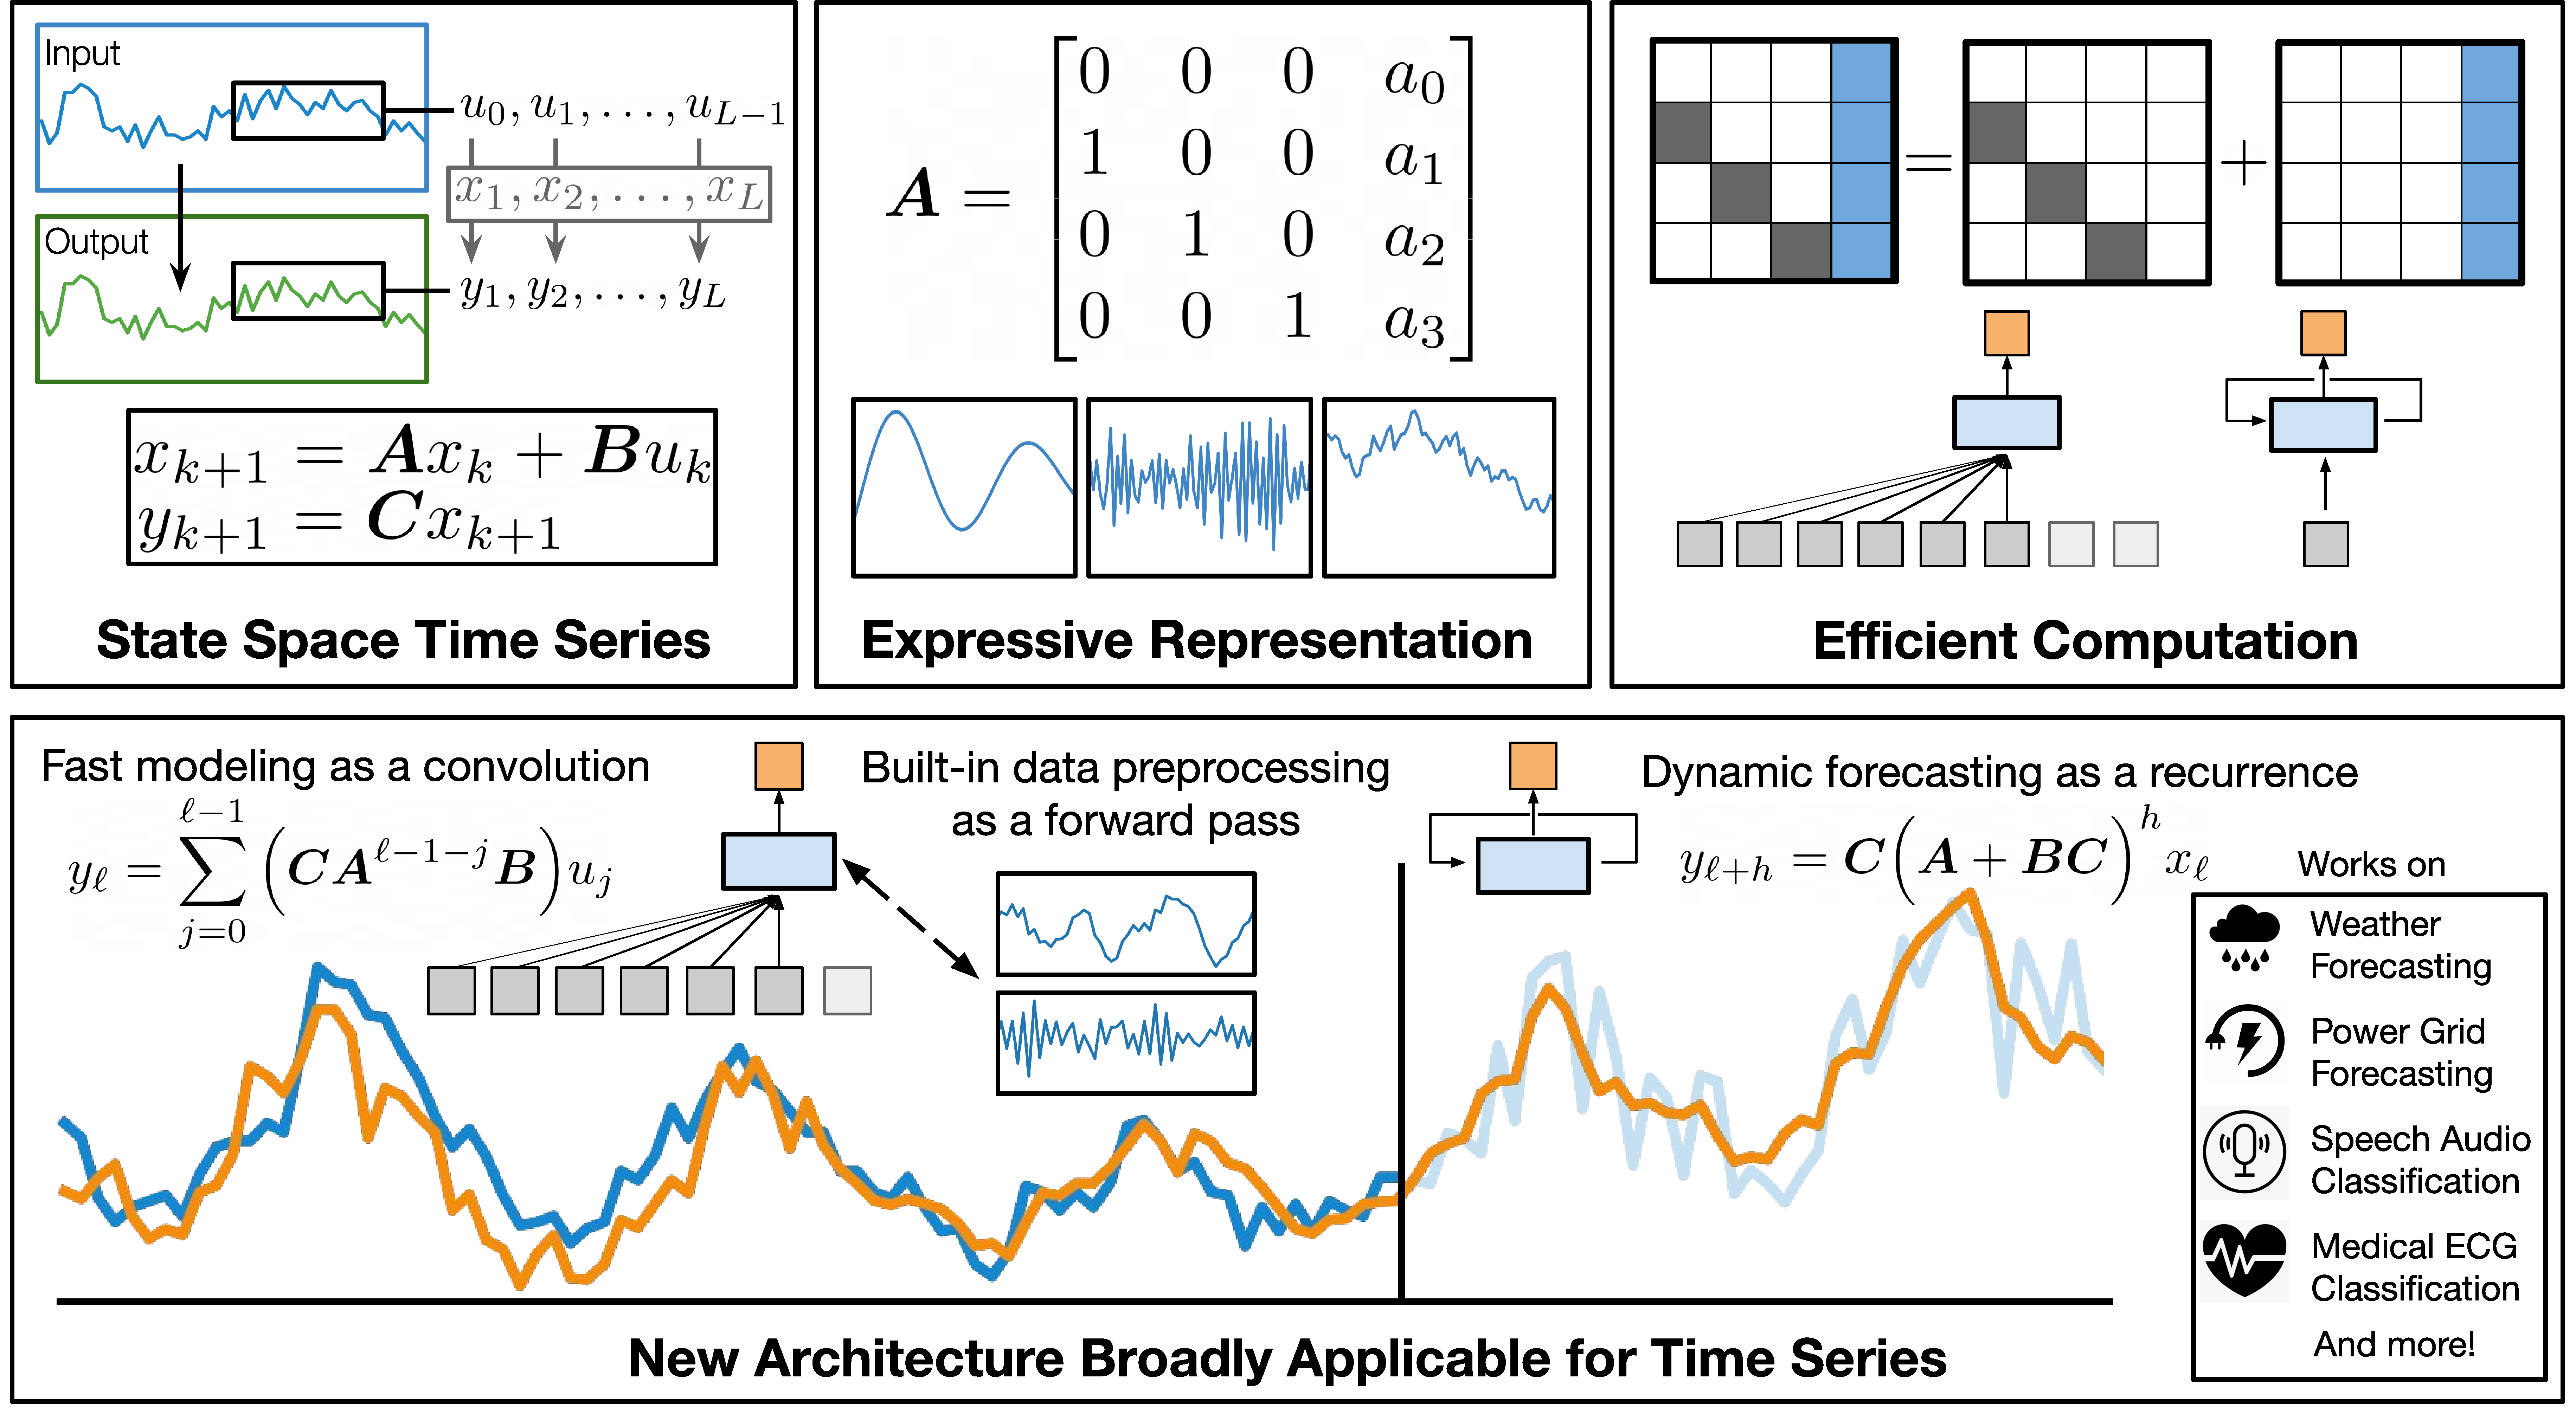
\includegraphics[width=1\textwidth]{_ICLR2023_paper/figures/time_series_ssm_use_this_2_levels_refactor1.pdf}
 \caption{We learn time series processes as state-space models (SSMs) (\textbf{top left}). We represent SSMs with the \textit{companion matrix}, which is a highly expressive representation for discrete time series  (\textbf{top middle}), and compute such SSMs efficiently as convolutions or recurrences via a shift + low-rank decomposition (\textbf{top right}). We use these SSMs to build \ourmethod{}, a new time series architecture broadly effective across tasks and domains (\textbf{bottom}).}
  \label{fig:overvew_fig1}
\end{figure}

% Our Method
%
% We thus propose \textbf{\ourmethod{}}, a new deep learning time series architecture. 
%
% Towards more effective time series modeling, 



We thus propose \textbf{\textsc{SpaceTime}}, a deep state-\textbf{space} architecture for effective \textbf{time} series modeling. 
% For more accurate forecasting and classification, 
To achieve this,
we focus on improving each criteria via three core contributions:

% \begin{enumerate}[itemsep=0.1pt,topsep=0pt,leftmargin=*]
\begin{enumerate}[topsep=0pt,leftmargin=*]
    \item For expressivity, our key idea and building block is a linear layer that models time series processes as \emph{state-space models} (SSMs) via the \emph{companion matrix} (Fig.~\ref{fig:overvew_fig1}). 
    We start with SSMs due to their connections to both classical time series analysis~\citep{kalman1960new, hamilton1994state} and recent deep learning advances~\citep{gu2021efficiently}. Classically, many time series models such as ARIMA and exponential smoothing (ETS) can be expressed as SSMs~\citep{box1970time, winters1960forecasting}. 
    Meanwhile, recent state-of-the-art deep sequence models~\citep{gu2021efficiently} have used SSMs to outperform Transformers and LSTMs on challenging long-range benchmarks~\citep{tay2020long}.
    % Meanwhile, recent SSM-based deep learning models~\citep{gu2021efficiently} have achieved state-of-the-art sequence modeling on challenging long-range benchmarks~\citep{tay2020long}. 
    Their primary innovations show how to formulate SSMs as neural network parameters that are practical to train. However, we find limitations with these deep SSMs for time series data. While we build on their advances, we prove that these prior SSM representations~\citep{ gu2021combining, gu2021efficiently, gupta2022diagonal}
    % cite these later: rangapuram2018, salinas2020deepar, lin2021ssdnet,
    cannot capture autoregressive processes fundamental for time series. We thus specifically propose the companion matrix representation for its expressive and memory-efficient properties. 
    We prove that the companion matrix SSM recovers fundamental autoregressive (AR) and smoothing processes modeled in classical techniques such as ARIMA and ETS, while only requiring $\mathcal{O}(d)$ memory to represent an $\mathcal{O}(d^2)$ matrix. 
    Thus, \ourmethod{} inherits the benefits of prior SSM-based sequence models, while introducing improved expressivity that 
    recovers fundamental time series processes
    % apture multiple AR processes and data preprocessing techniques 
    simply through its layer weights. 
    
    \item 
    % For forecasting over long horizons, we introduce a new ``closed-loop'' view of SSMs. Previous architectures apply the SSM in an ``open-loop'' fashion \citep{gu2021efficiently}, where the output is driven by the input sequence. 
    % However, to continuously forecast to long horizons, we require that the SSM has the ability to continue forecasting the signal in the absence of an input at those time steps. 
    % Inspired by classical closed-loop control~\citep{doyle2013feedback,aastrom2021feedback}, we propose a new variant of SSMs that explicitly models the next time-step input, which enables a multi-layer \ourmethod{} network to recurrently output long horizons.
    For forecasting long horizons, we introduce a new ``closed-loop'' view of SSMs. Prior deep SSM architectures either apply the SSM as an ``open-loop'' \citep{gu2021efficiently}, where fixed-length inputs necessarily generate same-length outputs, or use closed-loop autoregression where final layer outputs are fed through the \emph{entire} network as next-time-step inputs~\citep{goel2022s}. 
    We describe issues with both approaches in Sec.~\ref{sec:forecasting_ssm}, and instead achieve autogressive forecasting in a deep network with only a single SSM layer. We do so by explicitly training the SSM layer to predict its next time-step \emph{inputs}, alongside its usual outputs. This allows the SSM to recurrently generate its own future inputs that lead to desired outputs---\ie{} those that match an observed time series---so we can forecast over many future time-steps without explicit data inputs. 
    % This allows \ourmethod{} to generate its own final-layer inputs for outputting forecasts over many future time-steps.

    \item For efficiency, we introduce an algorithm for efficient training and inference with the companion matrix SSM. We 
    % first show how the companion SSM can be computed as both a convolution and a recurrence for layer-wise forward passes and forecasting respectively.  
    exploit the companion matrix's structure as a ``shift plus low-rank'' matrix, which allows us to reduce the time and space complexity for computing SSM hidden states and outputs from $\tilde{\mathcal{O}}(d \ell )$ to $\tilde{\mathcal{O}}(d + \ell)$ in SSM state size $d$ and input sequence length $\ell$. 
\end{enumerate}
% To subsequently build a full \ourmethod{} model, we simply stack together multiple layers---which each parametrize multiple companion matrix SSMs---into  a standard encoder-decoder architecture. 

% Simply stacking these layers together into a standard encoder-decoder architecture thus builds a highly expressive and efficient time series model.

In experiments, 
% we evaluate \ourmethod{} on extensive time series forecasting and classification tasks, and test if \ourmethod{}'s contributions empirically lead to (1) expressive time series modeling, (2) long-horizon forecasting, and (3) efficient training. 
%
we find \ourmethod{} consistently obtains state-of-the-art or near-state-of-the-art results, achieving best or second-best AUROC on 6 out of 7 ECG and audio speech time series classification tasks, and best mean-squared error (MSE) on 14 out of 16 Informer benchmark forecasting tasks~\citep{zhou2021informer}. \ourmethod{} also sets a new best average ranking across \numberMonashTasks{} tasks on the Monash benchmark~\citep{godahewa2021monash}.  
% 
We connect these gains with improvements on our three effective time series modeling criteria.  %
For expressivity, on synthetic ARIMA processes \ourmethod{} learns AR processes that prior deep SSMs cannot. 
%
% via extensive synthetics. As a controlled benchmark for expressiveness, we test how well popular architectures can fit standard AR processes, and find that \ourmethod{} best learns the true time series processes via its companion matrix SSM.
% compared to prior deep SSM representations.
%via visualizations of the process's ground-truth transfer function versus those parameterized by the trained SSM weights.
%
%
For long horizon forecasting, \ourmethod{} consistently outperforms prior state-of-the-art on the longest horizons by large margins. \ourmethod{} also generalizes better to \emph{new} horizons not used for training.
%
% validate that 
% We then validate (2) by showing that trained \ourmethod{}s generalize better to new horizons that models were not trained for. We also find that on the Informer benchmark, \ourmethod{} consistently outperforms alternatives on the longest evaluation horizons by the largest margins, up to $\textbf{X}$\% relative reduction in MSE for forecasting $\textbf{Y}$ time-steps.
%
% best RMSE on 25 out of 30 tasks from the diverse Monash benchmark~\citep{godahewa2021monash}.
% setting a new record among prior classical and deep learning approaches. 
% Moreover, we find that \ourmethod{} improves forecasts to arbitrary horizons (that it was not trained on) by \%XX on the Informer benchmark. 
For efficiency, on speed benchmarks \ourmethod{} obtains 73\% and 80\% relative wall-clock speedups over parameter-matched Transformers and LSTMs respectively, when training on real-world ETTh1 data.



%------------------------------------------------------------------------
\section{Serving Two Masters: Stability and Diversity with RpGAN \texorpdfstring{$+ R_1+R_2$}{R-1R-2}}
%---An Improved Training Objective \vk{title can be tweaked; i recommend naming your new loss}}
% James Tompkin: I wrote 'serving two masters'. Note that 'serving two masters' is inherently a religious label; in the bible, Matthew writes that one cannot serve two masters (only God). In the traditions of monarchy (to which our title alludes in the procession of kings), a king had divine right and so avoided this problem of serving two masters (to serve God and to serve one's king is to serve two masters, except once we establish that kings are divine then this problem goes away as the same master - God - is then being served). I am not religious.
\label{sec:loss}

In defining a GAN objective, we tackle two challenges: stability and diversity. Some previous work deals with stability~\cite{sg1,sg2,sg3} and other previous work deals with mode collapse \cite{rgan}. To make progress in both, we combine a stable method with a simple regularizer that is grounded by theory.


\subsection{Traditional GAN}
A traditional GAN~\cite{gan,nowozin2016f} is formulated as a minimax game between a discriminator (or critic) $D_\psi$ and a generator $G_\theta$. Given real data $x\sim p_\mathcal{D}$ and fake data $x\sim p_\theta$ produced by $G_\theta$, the most general form of a GAN is given by:
\begin{align}
\begin{split}
\label{eq:gan}
\mathcal{L}(\theta,\psi)=\mathbb{E}_{z\sim p_z}\left[f\left(  D_\psi(G_\theta(z))\right)\right]+\mathbb{E}_{x\sim p_\mathcal{D}}\left[f\left( -D_\psi(x) \right)\right]
\end{split}
\end{align}
\noindent where $G$ tries to minimize $\mathcal{L}$ while $D$ tries to maximize it. The choice of $f$ is flexible~\cite{lsgan,hingegan}. In particular, $f(t) = -\log(1+e^{-t})$ recovers the classic GAN by Goodfellow~\etal~\cite{gan}. For the rest of this work, this will be our choice of $f$~\cite{nowozin2016f}.

% It is shown that Eq.\ref{eq:gan} is actually convex if we can directly optimize $p_\theta$~\cite{gan,rpgan}. Though in practice, the empirical GAN loss moves fake samples past the decision boundary induced by $D$ rather than updating the density function $p_\theta$ directly. This turns out to be a much harder problem that is susceptible to two common failure cases: mode collapse/dropping\footnote{Mode collapse and mode dropping are technically two related yet distinct problems. We use these two terms interchangeably hereafter to refer to the general problem where $\supp p_\theta$ fails to fully cover $\supp p_\mathcal{D}$.} and non-convergence. \vk{Minor thing: could provide a bit more information (1 sentence) on mode dropping and collapse}
It has been shown that Equation~\ref{eq:gan} has convex properties when $p_\theta$ can be optimized directly~\cite{gan,rpgan}. However, in practical implementations, the empirical GAN loss typically shifts fake samples beyond the decision boundary set by $D$, as opposed to directly updating the density function $p_\theta$. This deviation leads to a significantly more challenging problem, characterized by susceptibility to two prevalent failure scenarios: mode collapse/dropping\footnote{While mode collapse and mode dropping are technically distinct issues, they are used interchangeably in this context to describe the common problem where $\supp(p_\theta)$ does not comprehensively cover $\supp(p_\mathcal{D})$. Mode collapse refers to the generator producing a limited diversity of samples (i.e., one image for the entire distribution), whereas mode dropping involves the generator failing to represent certain modes of the data distribution (ignoring entire subsets of the training distribution).} and non-convergence.



\subsection{Relativistic \texorpdfstring{$f$-GAN}{f-GAN}}
% We adopt relativistic pairing GAN (RpGAN) by Jolicoeur-Martineau~\etal~\cite{rgan} as the main GAN loss. 
% Sun~\etal showed that RpGAN is especially effective against mode dropping~\cite{rpgan} as the loss landscape of RpGAN contains no local minima that correspond to mode dropping solutions. 
% Next, we apply zero-centered gradient penalties~\cite{r1,r1r2} to RpGAN. Gradient penalty is a well known technique that stabilizes GAN training~\cite{wgan-gp,r1r2,r1} and has been proven to be crucial to GAN convergence~\cite{r1}. As our contribution to the theory, we follow Mescheder~\etal~\cite{r1} and prove that gradient-penalized RpGAN enjoys the same guarantee of local convergence as regularized classic GANs. In addition to theoretical guarantees, our empirical results suggest that gradient penalized RpGAN is sufficiently well-behaved, to the extent that allows us to remove all GAN tricks without encountering non-convergence or mode dropping.

We employ a slightly different minimax game named relativistic pairing GAN (RpGAN) by Jolicoeur-Martineau~\etal~\cite{rgan} to address mode dropping. The general RpGAN is defined as:
\begin{equation}
\label{eq:rpgan}
\mathcal{L}(\theta,\psi)=\mathbb{E}_{\substack{z\sim p_z\\x\sim p_\mathcal{D}}}\left[f\left(  D_\psi(G_\theta(z))-D_\psi(x) \right)\right]
\end{equation}
Although Eq.~\ref{eq:rpgan} differs only slightly from Eq.~\ref{eq:gan}, evaluating this critic difference has a fundamental impact on the landscape of $\mathcal{L}$. Since Eq.~\ref{eq:gan} merely requires $D$ to separate real and fake data, in the scenario where all real and fake data can be separated by a single decision boundary, the empirical GAN loss encourages $G$ to simply move all fake samples barely past this single boundary---this degenerate solution is what we observe as mode collapse/dropping. Sun~\etal~\cite{rpgan} characterize such degenerate solutions as bad local minima in the landscape of $\mathcal{L}$, and show that Eq.~\ref{eq:gan} has \emph{exponentially many} bad local minima. The culprit is the existence of a single decision boundary that naturally arises when real and fake data are considered in isolation. RpGAN introduces a simple solution by coupling real and fake data,~\ie a fake sample is critiqued by its realness \emph{relative to} a real sample, which effectively maintains a decision boundary in the neighborhood of \emph{each} real sample and hence forbids mode dropping. Sun~\etal~\cite{rpgan} show that the landscape of Eq.~\ref{eq:rpgan} contains no local minima that correspond to mode dropping solutions, and that every basin is a global minimum.


\subsection{Training Dynamics of RpGAN}
Although the RpGAN landscape result~\cite{rpgan} allows us to address mode dropping, the training dynamics of RpGAN have yet to be studied. The ultimate goal of Eq.~\ref{eq:rpgan} is to find the equilibrium $(\theta^*,\psi^*)$ such that $p_{\theta^*}=p_\mathcal{D}$ and $D_{\psi^*}$ is constant everywhere on $p_\mathcal{D}$. Sun~\etal~\cite{rpgan} show that $\theta^*$ is globally reachable along a non-increasing trajectory in the landscape of Eq.~\ref{eq:rpgan} under reasonable assumptions. However, the existence of such a trajectory does not necessarily mean that gradient descent will find it. Jolicoeur-Martineau~\etal show empirically that unregularized RpGAN does not perform well~\cite{rgan}. 

\vspace{1ex}
\noindent \textbf{Proposition~\upperRomannumeral{1}.} (Informal) \emph{Unregularized RpGAN does not always converge using gradient descent.}
%\vk{Propositions should ideally be made precise or in the worst case, say it's an informal statement (but then you still have to make it intuitively understandable)}
\vspace{1ex}

\noindent We confirm this proposition with a proof in Appendix B. 
% In summary, we follow Mescheder~\etal~\cite{r1} and inherit their DiracGAN counterexample to apply it to RpGAN. 
We show analytically that RpGAN does not converge for certain types of $p_\mathcal{D}$, such as ones that approach a delta distribution. Thus, further regularization is necessary to fill in the missing piece of a well-behaved loss.

\paragraph{Zero-centered gradient penalties.}
To tackle RpGAN non-convergence, we explore gradient penalties as the solution since it is proven that zero-centered gradient penalties (0-GP) facilitate convergent training for classic GANs~\cite{r1}. The two most commonly-used 0-GPs are $R_1$ and $R_2$:
\begin{equation}
\begin{aligned}
R_1(\psi)&=\frac{\gamma}{2}\mathbb{E}_{x\sim p_\mathcal{D}}\left[\left\| \nabla_x D_\psi \right \|^2\right]\\ 
R_2(\theta,\psi)&=\frac{\gamma}{2}\mathbb{E}_{x\sim p_\theta}\hspace{0.06cm}\left[\left\| \nabla_x D_\psi \right \|^2\right]
\end{aligned}
\end{equation}
$R_1$ penalizes the gradient norm of $D$ on real data, and $R_2$ penalizes the gradient norm of $D$ on fake data. Analysis on the training dynamics of GANs has thus far focused on local convergence~\cite{nagarajan2017gradient,gannum,r1},~\ie, whether the training at least converges when $(\theta,\psi)$ are in a neighborhood of $(\theta^*,\psi^*)$. In such a scenario, the convergence behavior can be analyzed~\cite{nagarajan2017gradient,gannum,r1} by examining the spectrum of the Jacobian of the gradient vector field $\left(-\nabla_\theta\mathcal{L},\nabla_\psi\mathcal{L} \right )$ at $(\theta^*,\psi^*)$. The key insight here is that when $G$ already produces the true distribution, we want $\nabla_x D=0$, so that $G$ is not pushed away from its optimal state, and thus the training does not oscillate. $R_1$ and $R_2$ impose such a constraint when $p_\theta=p_\mathcal{D}$. This also explains why earlier attempts at gradient penalties, such as the one-centered gradient penalty (1-GP) in WGAN-GP~\cite{wgan-gp}, fail to achieve convergent training~\cite{r1} as they still encourage $D$ to have a non-zero slope when $G$ has reached optimality.

Since the same insight also applies to RpGAN, 
we extend our previous analysis and show that:
% our goal is to extend the proof of Mescheder~\etal~\cite{r1} to RpGAN and show that:

\vspace{1ex}
\noindent \textbf{Proposition~\upperRomannumeral{2}.} (Informal) \emph{RpGAN with $R_1$ or $R_2$ regularization is locally convergent subject to similar assumptions as in} Mescheder~\etal~\cite{r1}.
\vspace{1ex}

In Appendix C, our proof similarly analyzes the eigenvalues of the Jacobian of the regularized RpGAN gradient vector field at $(\theta^*,\psi^*)$. We show that all eigenvalues have a negative real part; thus, regularized RpGAN is convergent in a neighborhood of $(\theta^*,\psi^*)$ for small enough learning rates~\cite{r1}.

%\vk{This paragraph is too verbose and feels like belongs to a prior work or discussion section} 
\paragraph{Discussion.}
Another line of work~\cite{r1r2} links $R_1$ and $R_2$ to instance noise~\cite{instancenoise} as its analytical approximation. Roth et al.~\cite{r1r2} showed that for the classic GAN~\cite{gan} by Goodfellow~\etal, $R_1$ approximates convolving $p_\mathcal{D}$ with the density function of $\mathcal{N}(0, \gamma I)$, up to additional weighting and a Laplacian error term. $R_2$ likewise approximates convolving $p_\theta$ with $\mathcal{N}(0, \gamma I)$ up to similar error terms. The Laplacian error terms from $R_1$, $R_2$ cancel when $D_\psi$ approaches $D_{\psi^*}$. We do not extend Roth~\etal's proof~\cite{r1r2} to RpGAN; however, this approach might provide complimentary insights to our work, which follows the strategy of Mescheder~\etal~\cite{r1}.

\subsection{A Practical Demonstration}

%\vk{i don't think that the rest of this section belongs in the methods section; i would first make it less verbose, then i would move large parts of it to the experiments, and i would summarize here in 1-2 sentences} 

We experiment with how well-behaved our loss is on StackedMNIST~\cite{pacgan} which consists of 1000 uniformly-distributed modes. The network is a small ResNet~\cite{resnet2} for $G$ and $D$ without any normalization layers~\cite{bn,gn,ln,in}.
Through the use of a pretrained MNIST classifier, we can explicitly measure how many modes of $p_\mathcal{D}$ are recovered by $p_\theta$. Furthermore, we can estimate the reverse KL divergence between the fake and real samples $D_\text{KL}\left(p_\theta\parallel p_\mathcal{D} \right)$ via the KL divergence between the categorical distribution of $p_\theta$ and the true uniform distribution.
\begin{figure}
\begin{floatrow}
\ffigbox{%
  \centering
  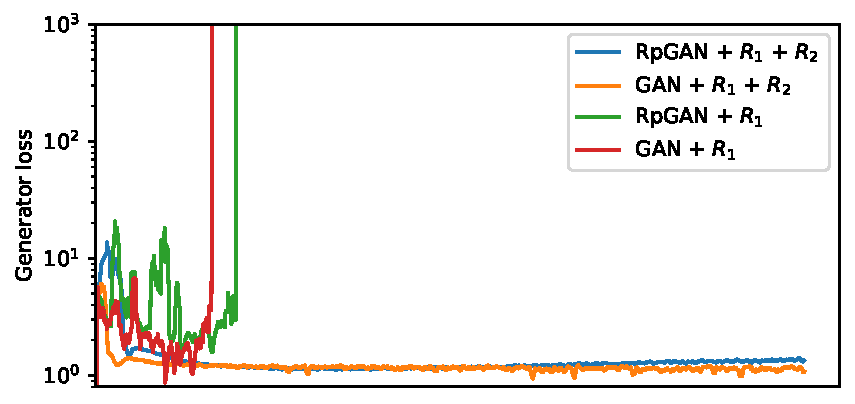
\includegraphics[width=0.48\textwidth]{figures/MNIST_loss.pdf}%
}{%
\caption{Generator $G$ loss for different objectives over training. Regardless of which objective is used, training diverges with only $R_1$ and succeeded with both $R_1$ and $R_2$. Convergence failure with only $R_1$ was noted by Lee et al.~\cite{vitgan}.}
\label{fig:mnist_loss_curve}
}
\capbtabbox{%
\centering
    \begin{tabular}{ l rrr }
        \toprule
        Loss & \# modes$\uparrow$ & $D_\text{KL}$$\downarrow$ \\
        \midrule
        RpGAN $+ R_1+R_2$ & $\mathbf{1000}$ & $\mathbf{0.0781}$ \\
        GAN $+ R_1+R_2$ & $693$ & $0.9270$ \\
        RpGAN $+ R_1$ & Fail & Fail \\
        GAN $+ R_1$ & Fail & Fail \\
        \bottomrule
    \end{tabular}
}{%
    \caption{StackedMNIST~\cite{pacgan} result for each loss function. The maximum possible mode coverage is 1000. ``Fail'' indicates that training diverged early on.}
    \label{tab:loss}
}
\end{floatrow}
\end{figure}

%For our initial experiments, we adopt a small ResNet~\cite{resnet2} architecture without any normalization layer~\cite{bn,gn,ln,in} for $G$ and $D$. 
A conventional GAN loss with $R_1$, as used by Mescheder et al.~\cite{r1} and the StyleGAN series~\cite{sg1, sg2, sg3}, diverges quickly (Fig.~\ref{fig:mnist_loss_curve}). Next, while theoretically sufficient for local convergence, RpGAN with only $R_1$ regularization is also unstable and diverges quickly\footnote{Varying $\gamma$ from 0.1 to 100 does not stabilize training.}. In each case, the gradient of $D$ on fake samples explodes when training diverges. With both $R_1$ and $R_2$, training becomes stable for both the classic GAN and RpGAN. Now stable, we can see that the classic GAN suffers from mode dropping, whereas RpGAN achieves full mode coverage (Tab.~\ref{tab:loss}) and reduces $D_\text{KL}$ from 0.9270 to 0.0781. As a point of contrast, StyleGAN~\cite{sg1,sg2,sg2ada,sg3} uses the minibatch standard deviation trick to reduce mode dropping, improving mode coverage from 857 to 881 on StackedMNIST\footnote{These numbers are from Karras~\etal~\cite{pggan}, Table 4. "857" corresponds to a low-capacity version of a progressive GAN and "881" adds the minibatch standard deviation trick. Further comparisons via loss curves are difficult since progressive GAN is a substantially different model than the small ResNet we use for this experiment.} and with barely any improvement on $D_\text{KL}$~\cite{pggan}.

%With training instability out of our way, we are ready to examine quantitatively how our new loss performs compared to existing work~\cite{r1,pggan,sg2}. While with $R_1$ and $R_2$ in conjunction training is successful for both the classic GAN~\cite{gan} and RpGAN~\cite{rgan}, we see in Table~\ref{tab:loss} that the classic GAN suffers from mode dropping. In contrast, RpGAN not only achieves full mode coverage, more notably, it drastically reduces $D_\text{KL}$ from 0.927 to 0.0781, indicating a considerably more faithful reconstruction of $p_\mathcal{D}$. 

% Instead of modifying the loss function, the StyleGAN family~\cite{sg1,sg2,sg2ada,sg3} relies on a trick called minibatch standard deviation~\cite{pggan} to combat mode dropping. It is shown in~\cite{pggan} that minibatch standard deviation can only slightly improve mode coverage from 857 to 881 on StackedMNIST and it shows barely any improvement on $D_\text{KL}$. 
% RpGAN in comparison improves mode coverage from 693 to 1000 and reduces $D_\text{KL}$ by one magnitude. 
%This shows that RpGAN is not only more principled against mode dropping in theory, but more effective in practice too. 
% We show in Section.\ref{sec:exp} that with architectural improvements in Section.\ref{sec:roadmap}, we can further improve $D_\text{KL}$ on StackedMNIST and even beat likelihood-based models. For the rest of this work, RpGAN $+ R_1+R_2$ will be our loss function.

% We start with RpGAN with only $R_1$ regularization since theoretically this is sufficient for local convergence. Contrary to our expectations, the training process utilizing this loss function exhibited significant instability and rapidly diverged. We experimented with various values of $\gamma$, ranging from 0.1 to 100; however, none succeeded in stabilizing the training. Furthermore, we explored integrating the conventional GAN loss combined with $R_1$, as commonly employed in the work of Mescheder et al.~\cite{r1} and the StyleGAN series~\cite{sg1, sg2, sg3}. Notably, this configuration led to even quicker divergence than the $R_1$ regularized RpGAN.
%To our surprise, training with this loss has been quite unstable and it diverges very quickly. We tried different $\gamma$ values ranging from 0.1 to 100 but none could prevent training from diverging. We also experiment with the combination of classic GAN and $R_1$, this is the widely adopted GAN loss in Mescheder~\etal~\cite{r1} and the StyleGAN family~\cite{sg1,sg2,sg3}, yet this loss diverges even faster than $R_1$ regularized RpGAN. 

% Upon closer inspection, we notice that the gradient of $D$ on fake samples explodes when training diverges. This motivates us to also apply $R_2$ regularization along with $R_1$, we see in Figure~\ref{fig:mnist_loss_curve} that with both $R_1$ and $R_2$, training becomes stable for both the classic GAN and RpGAN. 

$R_1$ alone is not sufficient for globally-convergent training. While a theoretical analysis of this is difficult, our small demonstration still provides insights into the assumptions of our convergence proof. 
In particular, the assumption that $(\theta,\psi)$ are sufficiently close to $(\theta^*,\psi^*)$ is highly unlikely early in training. In this scenario, if $D$ is sufficiently powerful, regularizing $D$ solely on real data is not likely to have much effect on $D$'s behavior on fake data and so training can fail due to an ill-behaved $D$ on fake data. This observation has been made by previous studies~\cite{r1gradexp, r1gradexpcvpr} specifically for empirical GAN training, that regularizing an empirical discriminator with only $R_1$ leads to gradient explosion on fake data due to the memorization of real samples.

% \vk{this is the key part that should be summarized in 1-2 sentences in this section: you find empirically and mathematically that both types of regularization are needed to make things work; then in the experiments section or in the appendix you provide results that show that it's the case}

Thus, the practical solution is to regularize $D$ on both real and fake data. The benefit of doing so can be viewed from the insight of Roth~\etal~\cite{r1r2}: that applying $R_1$ and $R_2$ in conjunction smooths both $p_\mathcal{D}$ and $p_\theta$ which makes learning easier than only smoothing $p_\mathcal{D}$. We also find empirically that with both $R_1$ and $R_2$ in place, $D$ tends to satisfy $\mathbb{E}_{x\sim p_\mathcal{D}}\left[\left\| \nabla_x D \right \|^2\right]\approx\mathbb{E}_{x\sim p_\theta}\left[\left\| \nabla_x D \right \|^2\right]$ even early in the training. Jolicoeur-Martineau~\etal~\cite{ganmmc} show that in this case $D$ becomes a maximum margin classifier---but if only one regularization term is applied, this does not hold. Additionally, having roughly the same gradient norm on real and fake data potentially reduces discriminator overfitting, as Fang~\etal~\cite{diggan} observe that the gradient norm on real and fake data diverges when $D$ starts to overfit.

% \vk{by the way, you will need a discussion of your regularization to other uses of this similar regularizer in the discussion or related work section}
% \begin{figure}
%     \centering
%     \includegraphics{figures/FID-vs-Params-Plot.eps}
%     \caption{This scatter-plot shows the FID performance of our model on FFHQ-256 vs the number of parameters when only trained for 5million steps}
%     \label{fig:fid-vs-params-ablation}
% \end{figure}


\section{A Roadmap to a New Baseline --- \modelName}
\label{sec:roadmap}

% \vk{What about naming the new GAN that is being proposed? SimpleGAN...?}\jt{R3GAN...?}

% \vk{My main comment about this section is that it reads like mix of methods and experiments: all the experimental details/results (e.g., we set the learning rate to $10^{-4}$) should be under experiments (but you can still describe the key important takeaways here, e.g., we need a smaller learning rate)}

The well-behaved RpGAN + $R_1$ + $R_2$ loss alleviates GAN optimization problems, and lets us proceed to build a minimalist baseline---\modelName---with recent network backbone advances in mind~\cite{convnext,metaformer}. Rather than simply state the new approach, we will draw out a roadmap from the StyleGAN2 baseline~\cite{sg2ada}. This model (Config A; identical to~\cite{sg2ada}) consists of a VGG-like~\cite{vgg} backbone for $G$, a ResNet $D$, a few techniques that facilitate style-based generation, and many tricks that serve as patches to the weak backbone. Then, we remove all non-essential features of StyleGAN2 (Config B), apply our loss function (Config C), and gradually modernize the network backbone (Config D-E).


We evaluate each configuration on FFHQ $256\times256$~\cite{sg1}. Network capacity is kept roughly the same for all configurations---both $G$ and $D$ have about 25\ M trainable parameters. Each configuration is trained until $D$ sees 5\ M real images. We inherit training hyperparameters (\eg, optimizer settings, batch size, EMA decay length) from Config A unless otherwise specified. We tune the training hyperparameters for our final model and show the converged result in Sec.~\ref{sec:exp}.

%\paragraph{StyleGAN2 (Config A).}This configuration is identical to the baseline~\cite{sg2ada} with the style-based generator and all tricks enabled.  

\vspace{-0.3cm}
\paragraph{Minimum baseline (Config B).}
\begin{wraptable}[21]{r}{8cm}
\vspace{-0.5cm}
\resizebox{1\linewidth}{!}{
\begin{tabular}{ l r c c c } 
\toprule
   & \multicolumn{1}{l}{Configuration}  & FID$\downarrow$                    & G \#params              & D \#params               \\ 
\midrule
A  & \multicolumn{1}{l}{StyleGAN2}  & 7.516                  & 24.767M                  & 24.001M                   \\
\midrule
B  & \multicolumn{1}{l}{Stripped StyleGAN2}                                                                                                                                                                                                                                                                                                                                                                                                                 &                        &                          &                           \\ 
   & \begin{tabular}[c]{@{}r@{}}\textcolor{red}{- $z$ normalization}\\ \textcolor{red}{- Minibatch stddev}\\ \textcolor{red}{- Equalized learning rate}\textcolor{red}{}\\\textcolor{red}{- Mapping network}\\ \textcolor{red}{- Style injection}\\ \textcolor{red}{- Weight mod / demod}\\ \textcolor{red}{- Noise injection}\\ \textcolor{red}{- Mixing regularization}\\ \textcolor{red}{- Path length regularization}\\ \textcolor{red}{- Lazy regularization}\textcolor{blue}{}\end{tabular} & \multirow{2}{*}{12.46} & \multirow{2}{*}{18.890M} & \multirow{2}{*}{23.996M}  \\ 
\midrule
C  & \multicolumn{1}{l}{Well-behaved Loss}                       &                        &                          &                           \\ 
 & \textcolor[rgb]{0,0.502,0.502}{+ RpGAN loss}                                                                                                                                                                                                                                                                                                                                                                                                                   & 11.77                                           & \multirow{2}{*}{18.890M} & \multirow{2}{*}{23.996M}                           \\ 
   & \textcolor[rgb]{0,0.502,0.502}{+ $R_2$ gradient penalty}                                                                                                                                                                                                                                                                                                                                                                                                & \multirow{1}{*}{11.65} &                          &                           \\ 
\midrule
D  & \multicolumn{1}{l}{ConvNeXt-ify pt.~1}                                                                                                                                                                                                                                                                                                                                                                                                                 &                        &                          &                           \\ 
 & \textcolor[rgb]{0,0.502,0.502}{+ ResNet-ify G $\&$ D}                                                                                                                                                                                                                                                                                                                                                                                                   & 10.17                  & 23.400M                  & \multirow{2}{*}{23.282M}  \\
   & \textcolor{red}{- Output skips}                                                                                                                                                                                                                                                                                                                                                                                                                         & 9.950 & 23.378M &                           \\ 
\midrule
E  & \multicolumn{1}{l}{ConvNeXt-ify pt.~2}                              &                        &                          &                           \\
 & \textcolor[rgb]{0,0.502,0.502}{+ ResNeXt-ify G $\&$ D}                                                                                                                                                                                                                                                                                                                                                                                                  & 7.507                  & 23.188M                  & 23.091M                   \\ 
   & \textcolor[rgb]{0,0.502,0.502}{+ Inverted bottleneck}                                                                                                                                         & 7.045 & 23.058M & 23.010M  \\ 
\bottomrule
\end{tabular}
}
\vspace{-0.25cm}
\caption{Effect of our simplification and modernization efforts evaluted on FFHQ-256.} 
\label{tab:roadmap}
\end{wraptable}

%To find the essential elements that contribute to StyleGAN2's success, 
We strip away all StyleGAN2 features, retaining only the raw network backbone and basic image generation capability. The features fall into three categories:
\begin{itemize}[leftmargin=10pt,itemsep=0pt,topsep=0pt]
\item Style-based generation: mapping network~\cite{sg1}, style injection~\cite{sg1}, weight modulation/demodulation~\cite{sg2}, noise injection~\cite{sg1}.
\end{itemize}\quad % JT: Weird but intential LaTeX
\begin{itemize}[leftmargin=10pt,itemsep=0pt,topsep=0pt]
\vspace{-0.25cm} % JT: Weird but intentional LaTeX
\item Image manipulation enhancements: mixing regularization~\cite{sg1}, path length regularization~\cite{sg2}.
\item Tricks: $z$ normalization~\cite{pggan}, minibatch stddev~\cite{pggan}, equalized learning rate~\cite{pggan}, lazy regularization~\cite{sg2}.
\end{itemize}

% Such features could be reintroduced as per application need (e.g., style injection). 
Following~\cite{sgxl,sg-t}, we reduce the dimension of $z$ to 64. The absence of equalized learning rate necessitates a lower learning rate, reduced from 2.5$\times$10\textsuperscript{-3} to 5$\times$10\textsuperscript{-5}. Despite a higher FID of 12.46 than Config-A, this simplified baseline produces reasonable sample quality and stable training. We compare this with DCGAN~\cite{dcgan}, an early attempt at image generation. Key differences include:
\begin{enumerate}[label=\alph*), noitemsep,topsep=0pt,leftmargin=24pt]
\item Convergent training objective with $R_1$ regularization.\label{item:convergent} 
\item Smaller learning rate, avoiding momentum optimizer (Adam $\beta_1=0$).\label{item:learning_rate} 
\item No normalization layer in $G$ or $D$.\label{item:normalization} 
\item Proper resampling via bilinear interpolation instead of strided (transposed) convolution.\label{item:resampling} 
\item Leaky ReLU in both $G$ and $D$, no tanh in the output layer of $G$.\label{item:activation} 
\item 4$\times$4 constant input for $G$, output skips for $G$, ResNet $D$.\label{item:input} 
\end{enumerate}

\textbf{Experimental findings from StyleGAN.} Violating \ref{item:convergent}, \ref{item:learning_rate}, or \ref{item:normalization} often leads to training failures.
%, contributing to the reputation that GANs as difficult to train. 
Gidel~\etal~\cite{ganmomentum} show that \emph{negative} momentum can improve GAN training dynamics. Since optimal negative momentum is another challenging hyperparameter, we do not use any momentum to avoid worsening GAN training dynamics. Studies suggest normalization layers harm generative models~\cite{sg2,edm2}. Batch normalization~\cite{bn} often cripples training due to dependencies across multiple samples, and is incompatible with $R_1$, $R_2$, or RpGAN that assume independent handling of each sample. Weaker data-independent normalizations~\cite{sg2,edm2} might help; we leave this for future work. Early GANs may succeed despite violating \ref{item:convergent} and \ref{item:normalization}, possibly constituting a full-rank solution~\cite{r1} to Eq.~\ref{eq:gan}.

Violations of \ref{item:resampling} or \ref{item:activation} do not significantly impair training stability but negatively affect sample quality. Improper transposed convolution can cause checkerboard artifacts, unresolved even with subpixel convolution~\cite{subpixel} or carefully tuned transposed convolution unless a low-pass filter is applied. Interpolation methods avoid this issue, varying from nearest neighbor~\cite{pggan} to Kaiser filters~\cite{sg3}. We use bilinear interpolation for simplicity. For activation functions, smooth approximations of (leaky) ReLU, such as Swish~\cite{swish}, GELU~\cite{gelu}, and SMU~\cite{smu}, worsen FID. PReLU~\cite{prelu} marginally improves FID but increases VRAM usage, so we use leaky ReLU.

All subsequent configurations adhere to \ref{item:convergent} through \ref{item:activation}. Violation of \ref{item:input} is acceptable as it pertains to the network backbone of StyleGAN2~\cite{sg2}, modernized in Config D and E.

% \paragraph{Minimum baseline (Config B).}
% To elucidate the implementation details that contribute to the success of StyleGAN2, we remove all the StyleGAN2 features until only the raw network backbone and basic image generation capability are retained. The list of removed features can be placed into three categories:
% \begin{itemize}
%     \item Style-based generation: mapping network~\cite{sg1}, style injection~\cite{sg1}, weight modulation / demodulation~\cite{sg2}, noise injection~\cite{sg1}.
%     \item Image manipulation enhancements: mixing regularization~\cite{sg1}, path length regularization~\cite{sg2}.
%     \item Tricks: $z$ normalization~\cite{pggan}, minibatch stddev~\cite{pggan}, equalized learning rate~\cite{pggan}, lazy regularization~\cite{sg2}.
% \end{itemize}
% The first two categories are technically orthogonal to our work; we remove them along with the tricks as our goal is to build a minimalist baseline and they can be reintroduced to our model in the future. \aaron{For this work, we want to keep our baseline as simple as possible, and demonstrate that many of these additions are not necessary for training a state of the art GAN. Instead, we ask what the simplest architecture one can design that can be used to train a GAN.}\vk{Do you include back the things you remove? Curious why / why not} Following~\cite{sgxl,sg-t}, we decrease the dimension of $z$ to 64. The removal of equalized learning rate necessitates a significantly lower learning rate and we decrease the learning rate from $2.5\times10^{-3}$ to $5\times10^{-5}$, any higher learning rate cripples training. This highly simplified baseline, despite achieving a considerably worse FID of 12.46, produces quite reasonable sample quality and training is stable. We compare this baseline against DCGAN~\cite{dcgan}, a barely working early GAN attempt at image generation. Notable differences include:
% \begin{enumerate}[label=\alph*)]
%     \item Convergent training objective with $R_1$ regularization.
%     \item Smaller learning rate, not using a momentum optimizer (Adam $\beta_1=0$).
%     \item Neither $G$ nor $D$ uses any normalization layer.
%     \item Proper resampling via bilinear interpolation instead of strided (transposed) convolution.
%     \item Leaky ReLU in both $G$ and $D$, no tanh in the output layer of $G$.
%     \item $4\times4$ constant input for $G$, output skips for $G$, ResNet $D$.
% \end{enumerate}

% \vk{Part B too verbose and many of these details can be in appendix  or removed }
% Our experiments show that any violation of a), b), or c) can easily lead to training failures, and these violations likely earned GANs the reputation of being hard to train. Gidel~\etal~\cite{ganmomentum} show that momentum not only should be avoided for GAN optimization, but \emph{negative} momentum might even improve GAN training dynamics. Since the optimal negative momentum is another hard to tune hyperparameter, we simply do not use any momentum to at least not worsen the GAN training dynamics. Recent studies~\cite{sg2,edm2} on GANs and diffusion models show that normalization layers harm generative models. Batch normalization~\cite{bn} in particular often cripples training as it establishes dependency across multiple samples and it is therefore incompatible with $R_1$, $R_2$ or RpGAN, all of which assume that the networks handle each sample independently. Although weaker data-independent normalizations~\cite{sg2,edm2} might still help, we leave these as future work and do not employ any normalization technique. A curious case with many early GANs is that the simultaneous violation of a) and c) (\eg using batch normalization and not using any gradient penalty) occasionally leads to successful training. One possible explanation is that this might constitute a full-rank solution~\cite{r1} to Eq.\ref{eq:gan} which is also locally convergent.

% Violations of d) or e) do not impair training stability much, however, these violations are detrimental to sample quality. Upsampling with improper transposed convolution can result in imbalanced overlaps between pixels which lead to checkerboard artifacts. The artifacts cannot be fully resolved even when the imbalanced overlap problem is eliminated by subpixel convolution~\cite{subpixel} or carefully tuned transposed convolution unless a proper low-pass filter is applied. Interpolation in comparison avoids such failure directly from the source. The choice of the interpolation method varies wildly in previous works, from naive approaches such as nearest neighbor~\cite{pggan} to advanced resampling techniques such as Kaiser filters~\cite{sg3}, we retain the choice of bilinear interpolation for simplicity. For the activation function, we experiment with various smooth approximations of (leaky) ReLU including Swish~\cite{swish}, GELU~\cite{gelu} and SMU~\cite{smu}, all of which deteriorate FID considerably. The only activation function we find to marginally improve FID is PReLU~\cite{prelu}, however, the tiny improvement does not justify the considerably higher VRAM usage, and therefore we settle for leaky ReLU.

% For all subsequent configurations, we ensure compliance to a) through e). We are free to violate f) as this is merely the network backbone adopted by StyleGAN2~\cite{sg2} and we modernize the backbone in Config D and E.

\vspace{-0.3cm}
\paragraph{Well-behaved loss function (Config C).}
% Given the simplified baseline, we move on to the modernization part of the roadmap. We first modernize the loss function so that the representation power of modern network backbones will not be compromised by GAN optimization difficulties. 
We use the loss function proposed in Section~\ref{sec:loss} and this reduces FID to 11.65. We hypothesize that the network backbone in Config B is the limiting factor. 
% and expect more drastic improvements as further modernization takes place.


\begin{figure*}[t]%
\centering\footnotesize%
 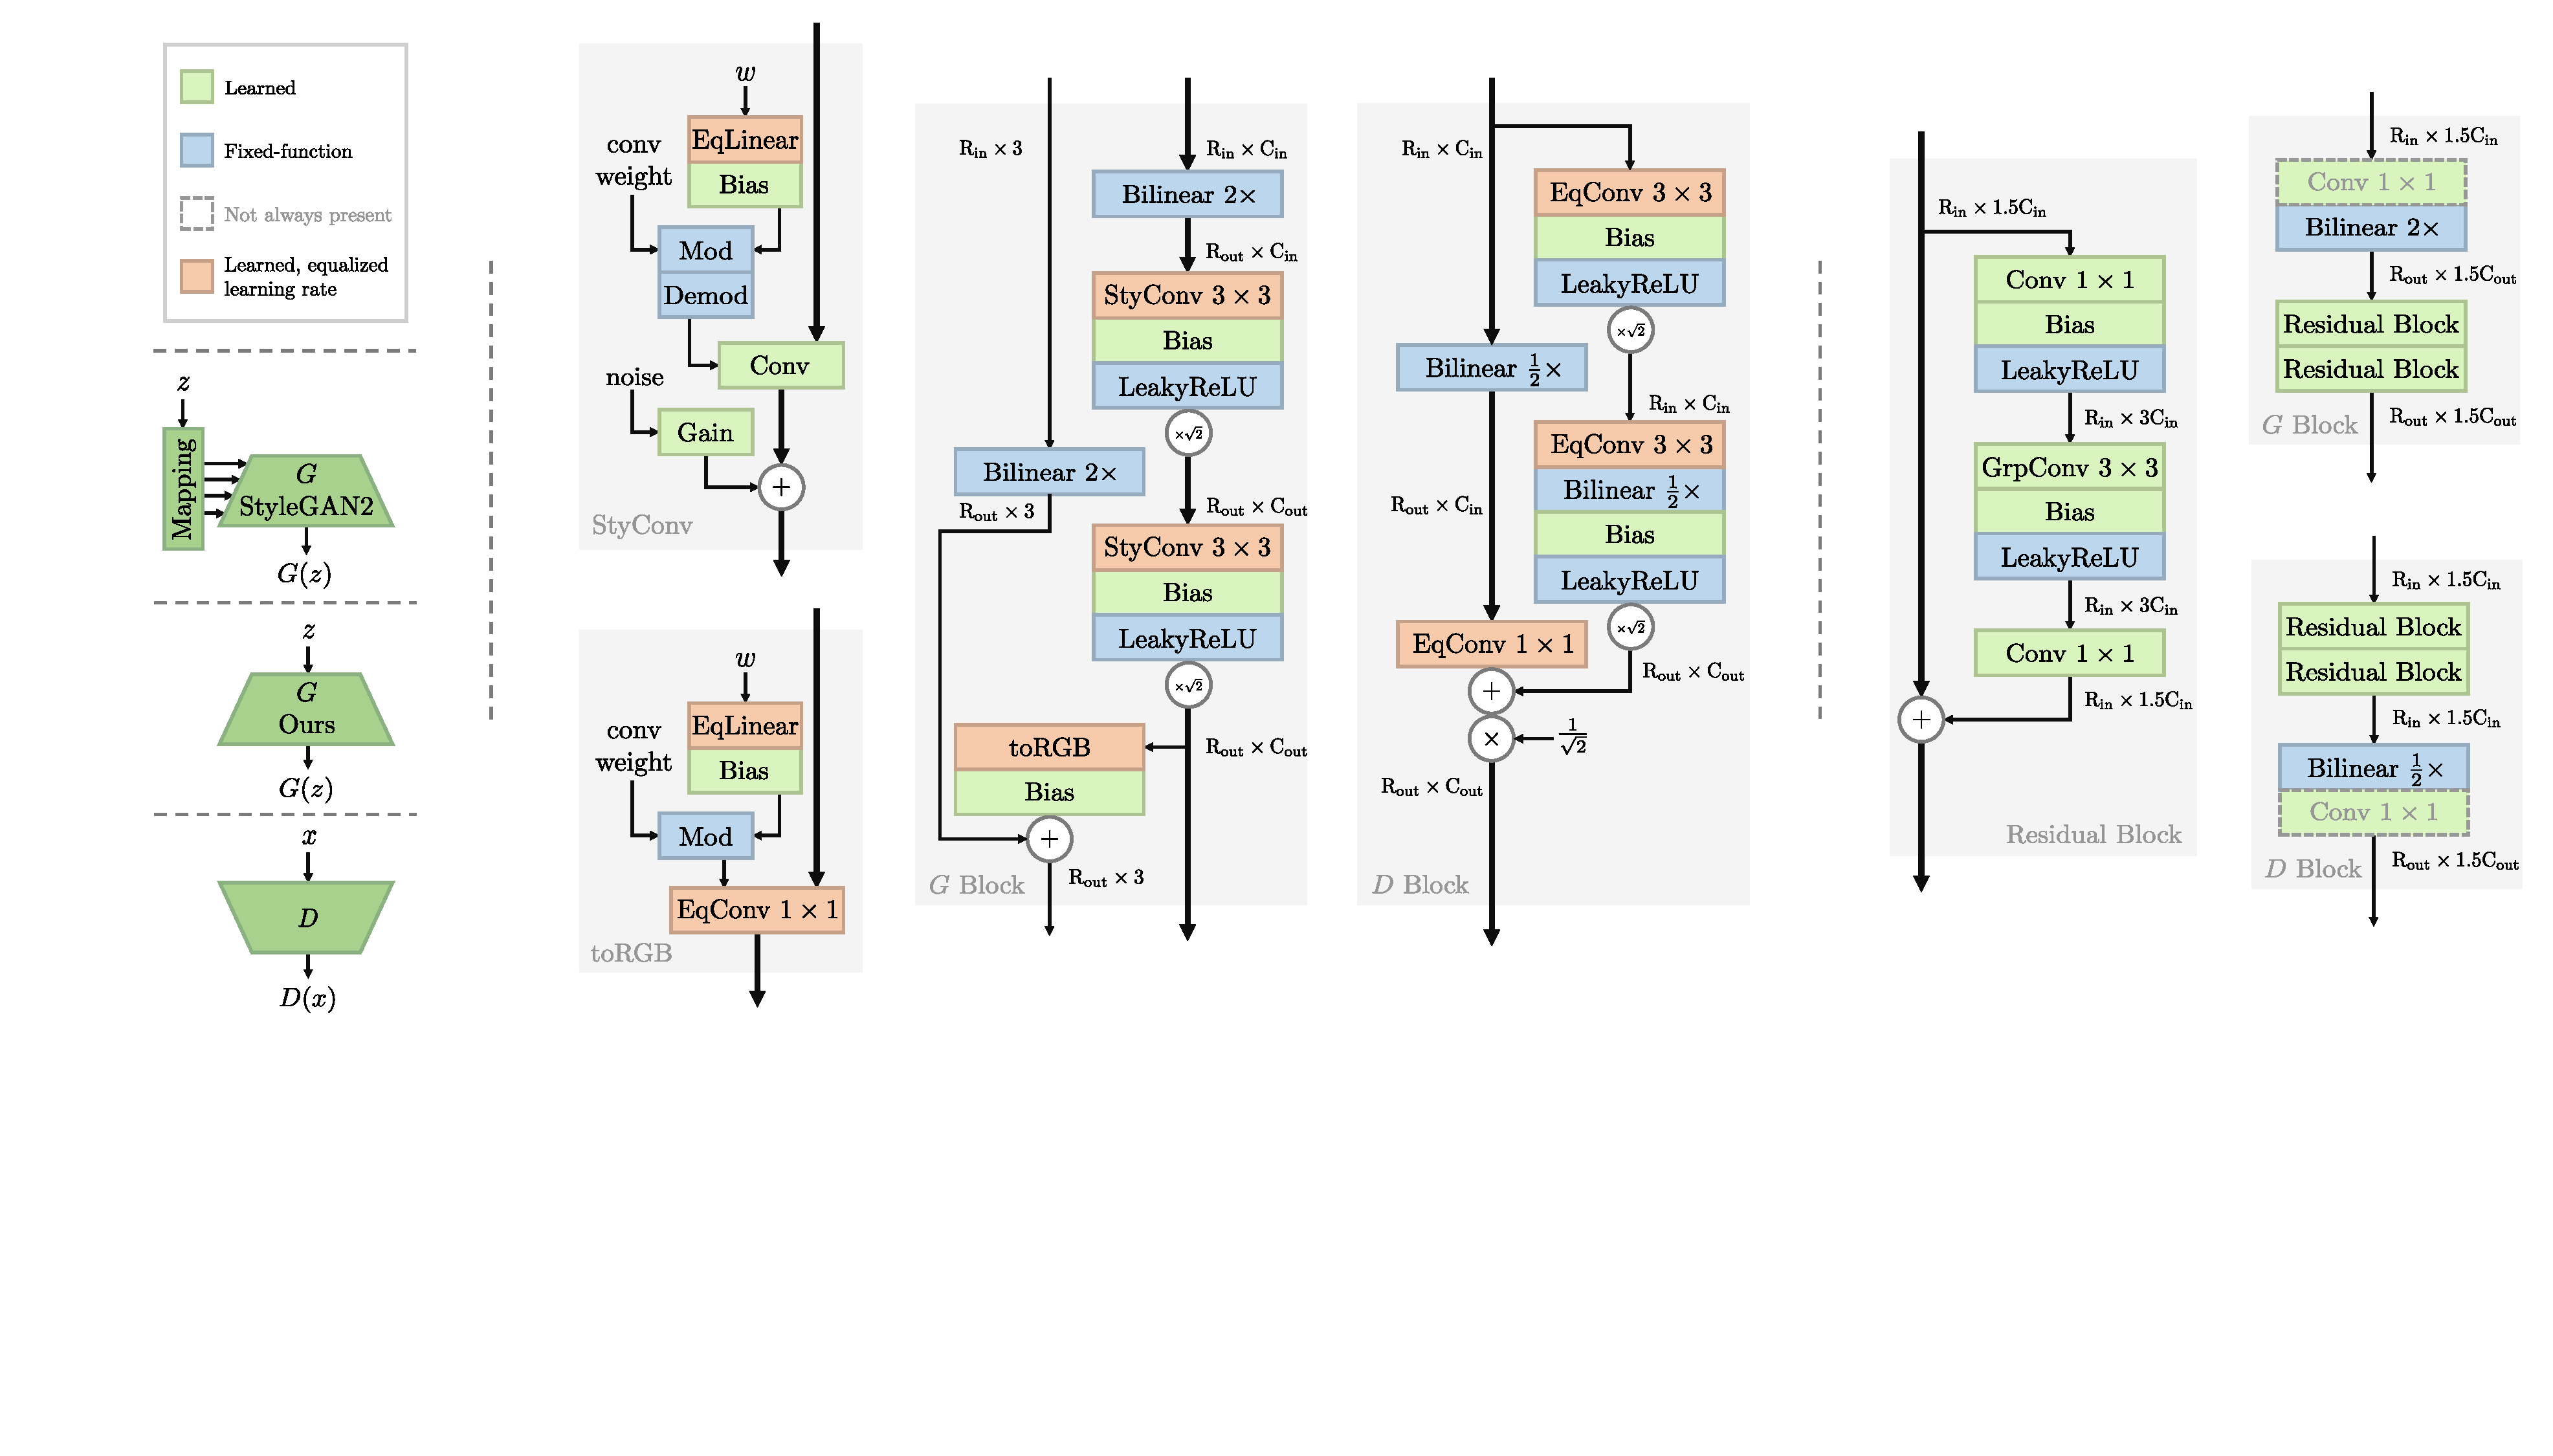
\includegraphics[width=\linewidth,clip,trim={3.5cm 11.5cm 0cm 0cm}]{figures/arch.pdf}\\%
\makebox[0.144\linewidth]{(a) Overall view}\hfill%
\makebox[0.562\linewidth]{(b) StyleGAN2 architecture blocks~\cite{sg2} (Config A)}\hfill%
\makebox[0.294\linewidth]{(c) Ours (Config E)}\hfill%
\vspace{0.5mm}
\caption{\label{fig:network}%
\textbf{Architecture comparison.}
For image generation, $G$ and $D$ are often both deep ConvNets with either partially or fully symmetric architectures.
\textbf{(a)}
StyleGAN2~\cite{sg2} $G$ uses a network to map noise vector $z$ to an intermediate style space $\mathcal{W}$. We use a traditional generator as style mapping is not necessary for a minimal working model.
\textbf{(b)}
StyleGAN2's building blocks have intricate layers but are themselves simple, with a ConvNet architecture from 2015~\cite{alexnet,vgg,resnet}. ResNet's identity mapping principle is also violated in the discriminator.
\textbf{(c)}
We remove tricks and modernize the architecture. Our design has clean layers with a more powerful ConvNet architecture.
}%
\vspace{-0.3cm}%
\end{figure*}

\vspace{-0.3cm}
\paragraph{General network modernization (Config D).}
First, we apply the 1-3-1 bottleneck ResNet architecture~\cite{resnet,resnet2} to both $G$ and $D$. This is the direct ancestor of all modern vision backbones~\cite{convnext,metaformer}. 
% However, rather than precisely replicating the architecture in~\cite{resnet2}, 
We also incorporate principles discovered in Config B and various modernization efforts from ConvNeXt~\cite{convnext}. We categorize the roadmap of ConvNeXt as follows:
% \begin{enumerate}[label=\roman*)]
%     \item Consistently beneficial: 1) increased width with depthwise conv. 2) inverted bottleneck. 3) fewer activation functions. 4) separate resampling layers.
%     \item Negligible performance gain: 1) large kernel depthwise conv with fewer channels. 2) replacing ReLU with GELU. 3) fewer normalization layers. 4) replacing batch norm with layer norm.
%     \item Irrelevant to our problem setting: 1) improved training recipe. 2) stage ratio. 3) "patchify" stem.
% \end{enumerate}
% % We are interested in applying i) to our model, among which i.3) and i.4) are applicable to the classic ResNet. We leave i.1) and i.2) for Config E. Much of ii) were introduced merely for the sake of mimicking vision transformers~\cite{swin,vit} even though they fail to bring any significant improvement~\cite{convnext}. ii.3) and ii.4) are inapplicable since we do not use any normalization layer following principle c). ii.2) is directly at odds with our finding that GELU deteriorates GAN performance, and we use leaky ReLU as in principle e). Liu~\etal put heavy emphasis on using large conv kernels (ii.1)~\cite{convnext}, however this results in slightly but consistently worse performance than using wider $3\times3$ conv layers and we therefore do not employ this design choice of ConvNeXt.

% We aim to apply i) to our model, specifically i.3) and i.4) for the classic ResNet, while reserving i.1) and i.2) for Config E. Many aspects of ii) were introduced merely to mimic vision transformers~\cite{swin,vit} without yielding significant improvements~\cite{convnext}. ii.3) and ii.4) are inapplicable due to our avoidance of normalization layers following principle c). ii.2) contradicts our finding that GELU deteriorates GAN performance, thus we use leaky ReLU per principle e). Liu~\etal emphasize large conv kernels (ii.1)~\cite{convnext}, but this results in slightly worse performance compared to wider $3\times3$ conv layers, so we do not adopt this ConvNeXt design choice.
%
\begin{enumerate}[label=\roman*., itemsep=1pt,leftmargin=12pt,topsep=0pt,parsep=1pt]
    \item Consistently beneficial: \begin{enumerate*}[label=\theenumi\arabic*), ref=\arabic*, before=\unskip{ }, itemjoin={{, }}, itemjoin*={{, and }}]
        \item\label{item:i1} increased width with depthwise convolution
        \item\label{item:i2} inverted bottleneck
        \item\label{item:i3} fewer activation functions
        \item\label{item:i4} separate resampling layers.
    \end{enumerate*}
    \item Negligible performance gain: \begin{enumerate*}[label=\theenumi\arabic*), ref=\arabic*, before=\unskip{ }, itemjoin={{, }}, itemjoin*={{, and }}]
        \item\label{item:ii1} large kernel depthwise conv.~with fewer channels
        \item\label{item:ii2} swap ReLU with GELU
        \item\label{item:ii3} fewer normalization layers
        \item\label{item:ii4} swap batch norm.~with layer norm.
    \end{enumerate*}
    \item Irrelevant to our setting: \begin{enumerate*}[label=\theenumi\arabic*), ref=\arabic*, before=\unskip{ }, itemjoin={{, }}, itemjoin*={{, and }}]
        \item\label{item:iii1} \hspace{-0.1cm}improved training recipe
        \item\label{item:iii2} \hspace{-0.1cm}stage ratio
        \item\label{item:iii3} \hspace{-0.1cm}`patchify' stem.
    \end{enumerate*}
\end{enumerate}

We aim to apply i) to our model, specifically i.\ref{item:i3} and i.\ref{item:i4} for the classic ResNet, while reserving i.\ref{item:i1} and i.\ref{item:i2} for Config E. Many aspects of ii) were introduced merely to mimic vision transformers~\cite{swin,vit} without yielding significant improvements~\cite{convnext}. ii.\ref{item:ii3} and ii.\ref{item:ii4} are inapplicable due to our avoidance of normalization layers following principle \ref{item:normalization}. ii.\ref{item:ii2} contradicts our finding that GELU deteriorates GAN performance, thus we use leaky ReLU per principle \ref{item:activation}. Liu~\etal emphasize large conv.~kernels (ii.\ref{item:ii1})~\cite{convnext}, but this results in slightly worse performance compared to wider 3$\times$3 conv.~layers, so we do not adopt this ConvNeXt design choice.

\paragraph{Neural network architecture details.} Given i.\ref{item:i3}, i.\ref{item:i4}, and principles \ref{item:normalization}, \ref{item:resampling}, and \ref{item:activation}, we can replace the StyleGAN2 backbone with a modernized ResNet. We use a fully symmetric design for $G$ and $D$ with 25\ M parameters each, comparable to Config-A. The architecture is minimalist: each resolution stage has one transition layer and two residual blocks. The transition layer consists of bilinear resampling and an optional 1$\times$1 conv.~for changing spatial size and feature map channels. The residual block includes five operations: Conv1$\times$1$\rightarrow$ Leaky ReLU $\rightarrow$ Conv3$\times$3$\rightarrow$ Leaky ReLU $\rightarrow$ Conv1$\times$1, with the final Conv1$\times$1 having no bias term. For the 4$\times$4 resolution stage, the transition layer is replaced by a basis layer for $G$ and a classifier head for $D$. The basis layer, similar to StyleGAN~\cite{sg1,sg2}, uses 4$\times$4 learnable feature maps modulated by $z$ via a linear layer. The classifier head uses a global 4$\times$4 depthwise conv.~to remove spatial extent, followed by a linear layer to produce $D$'s output. We maintain the width ratio for each resolution stage as in Config A, making the stem width 3$\times$ as wide due to the efficient 1$\times$1 conv. The 3$\times$3 conv.~in the residual block has a compression ratio of 4, following~\cite{resnet,resnet2}, making the bottleneck width 0.75$\times$ as wide as Config A.
%Given i.3), i.4) and principles c), d), and e), we are now ready to replace the StyleGAN2 backbone with a modernized ResNet. We adopt a fully symmetric design for $G$ and $D$, and make the model size comparable to Config A, both $G$ and $D$ have approximately 25M parameters. We keep the architecture as minimalist as possible, for each resolution stage, we have one transition layer and two residual blocks. The transition layer consists of bilinear resampling and an optional $1\times1$ conv that allows us to change the spatial size and the number of channels of the feature maps. The residual block contains five consecutive operations on the residual branch: Conv$1\times1\rightarrow$ Leaky ReLU $\rightarrow$ Conv$3\times3\rightarrow$ Leaky ReLU $\rightarrow$ Conv$1\times1$, and the final Conv$1\times1$ has no bias term. For the $4\times4$ resolution stage, the transition layer is replaced by a basis layer for $G$ and a classifier head for $D$. The basis layer resembles the const input of StyleGAN~\cite{sg1,sg2} where a set of $4\times4$ learnable feature maps are modulated by $z$ via a linear layer. The classifier head first removes the spatial extent of the feature maps with a global $4\times4$ depthwise conv; the features are then fed to a linear layer to produce the output of $D$. We keep the width ratio for each resolution stage the same as Config A, and we are able to make the stem width $3\times$ as wide as Config A given the same model size thanks to the more efficient $1\times1$ conv. The compression ratio for the $3\times3$ conv in the residual block is set to 4 following~\cite{resnet,resnet2}, this makes the bottleneck width $0.75\times$ as wide as Config A.

% The lack of normalization necessitates more careful initialization for ResNet to avoid variance explosion. We apply fix-up initialization~\cite{fixup} to our modernized networks to remedy this. Concretely, we zero-initialize the last conv layer in each residual block, and scale down the initialization of the other two conv layers in the residual block by $L^{-0.25}$ where $L$ is the number of residual blocks in the network. We do not employ any other trick from fixup~\cite{fixup} such as applying excessive bias terms and the use of a scalar multiplier. The new network architecture and the initialization scheme allow us to raise the learning rate to $1\times10^{-4}$ without encountering training instability.
To avoid variance explosion due to the lack of normalization, we employ fix-up initialization~\cite{fixup}: 
%for our modernized networks: 
We zero-initialize the last convolutional layer in each residual block and scale down the initialization of the other two convolutional layers in the block by $L^{-0.25}$, where $L$ is the number of residual blocks. We avoid other fix-up tricks, such as excessive bias terms and a learnable multiplier.

% We show that removing all these architectural modifications of the original StyleGAN mildly harms performance, but not as much as one might expect in~\ref{sub:arc-experiments}. Furthermore, removing some components actually benefits FID.


% \begin{figure}
%     \centering
%     \includegraphics[width=0.25\linewidth]{example-image-a}

%     \caption{Swirl Figure. We show our model matches performance on Gaussian toy example. \aaron{Are we still doing a toy example}]}
%     \label{fig:enter-label}
% \end{figure}

% \begin{figure}
%     \centering
%     \includegraphics[width=0.25\linewidth]{example-image-b}
%     \caption{k-NN decision barrier. Intuitive example}
%     \label{fig:enter-label}
% \end{figure}

% \begin{figure*}
%     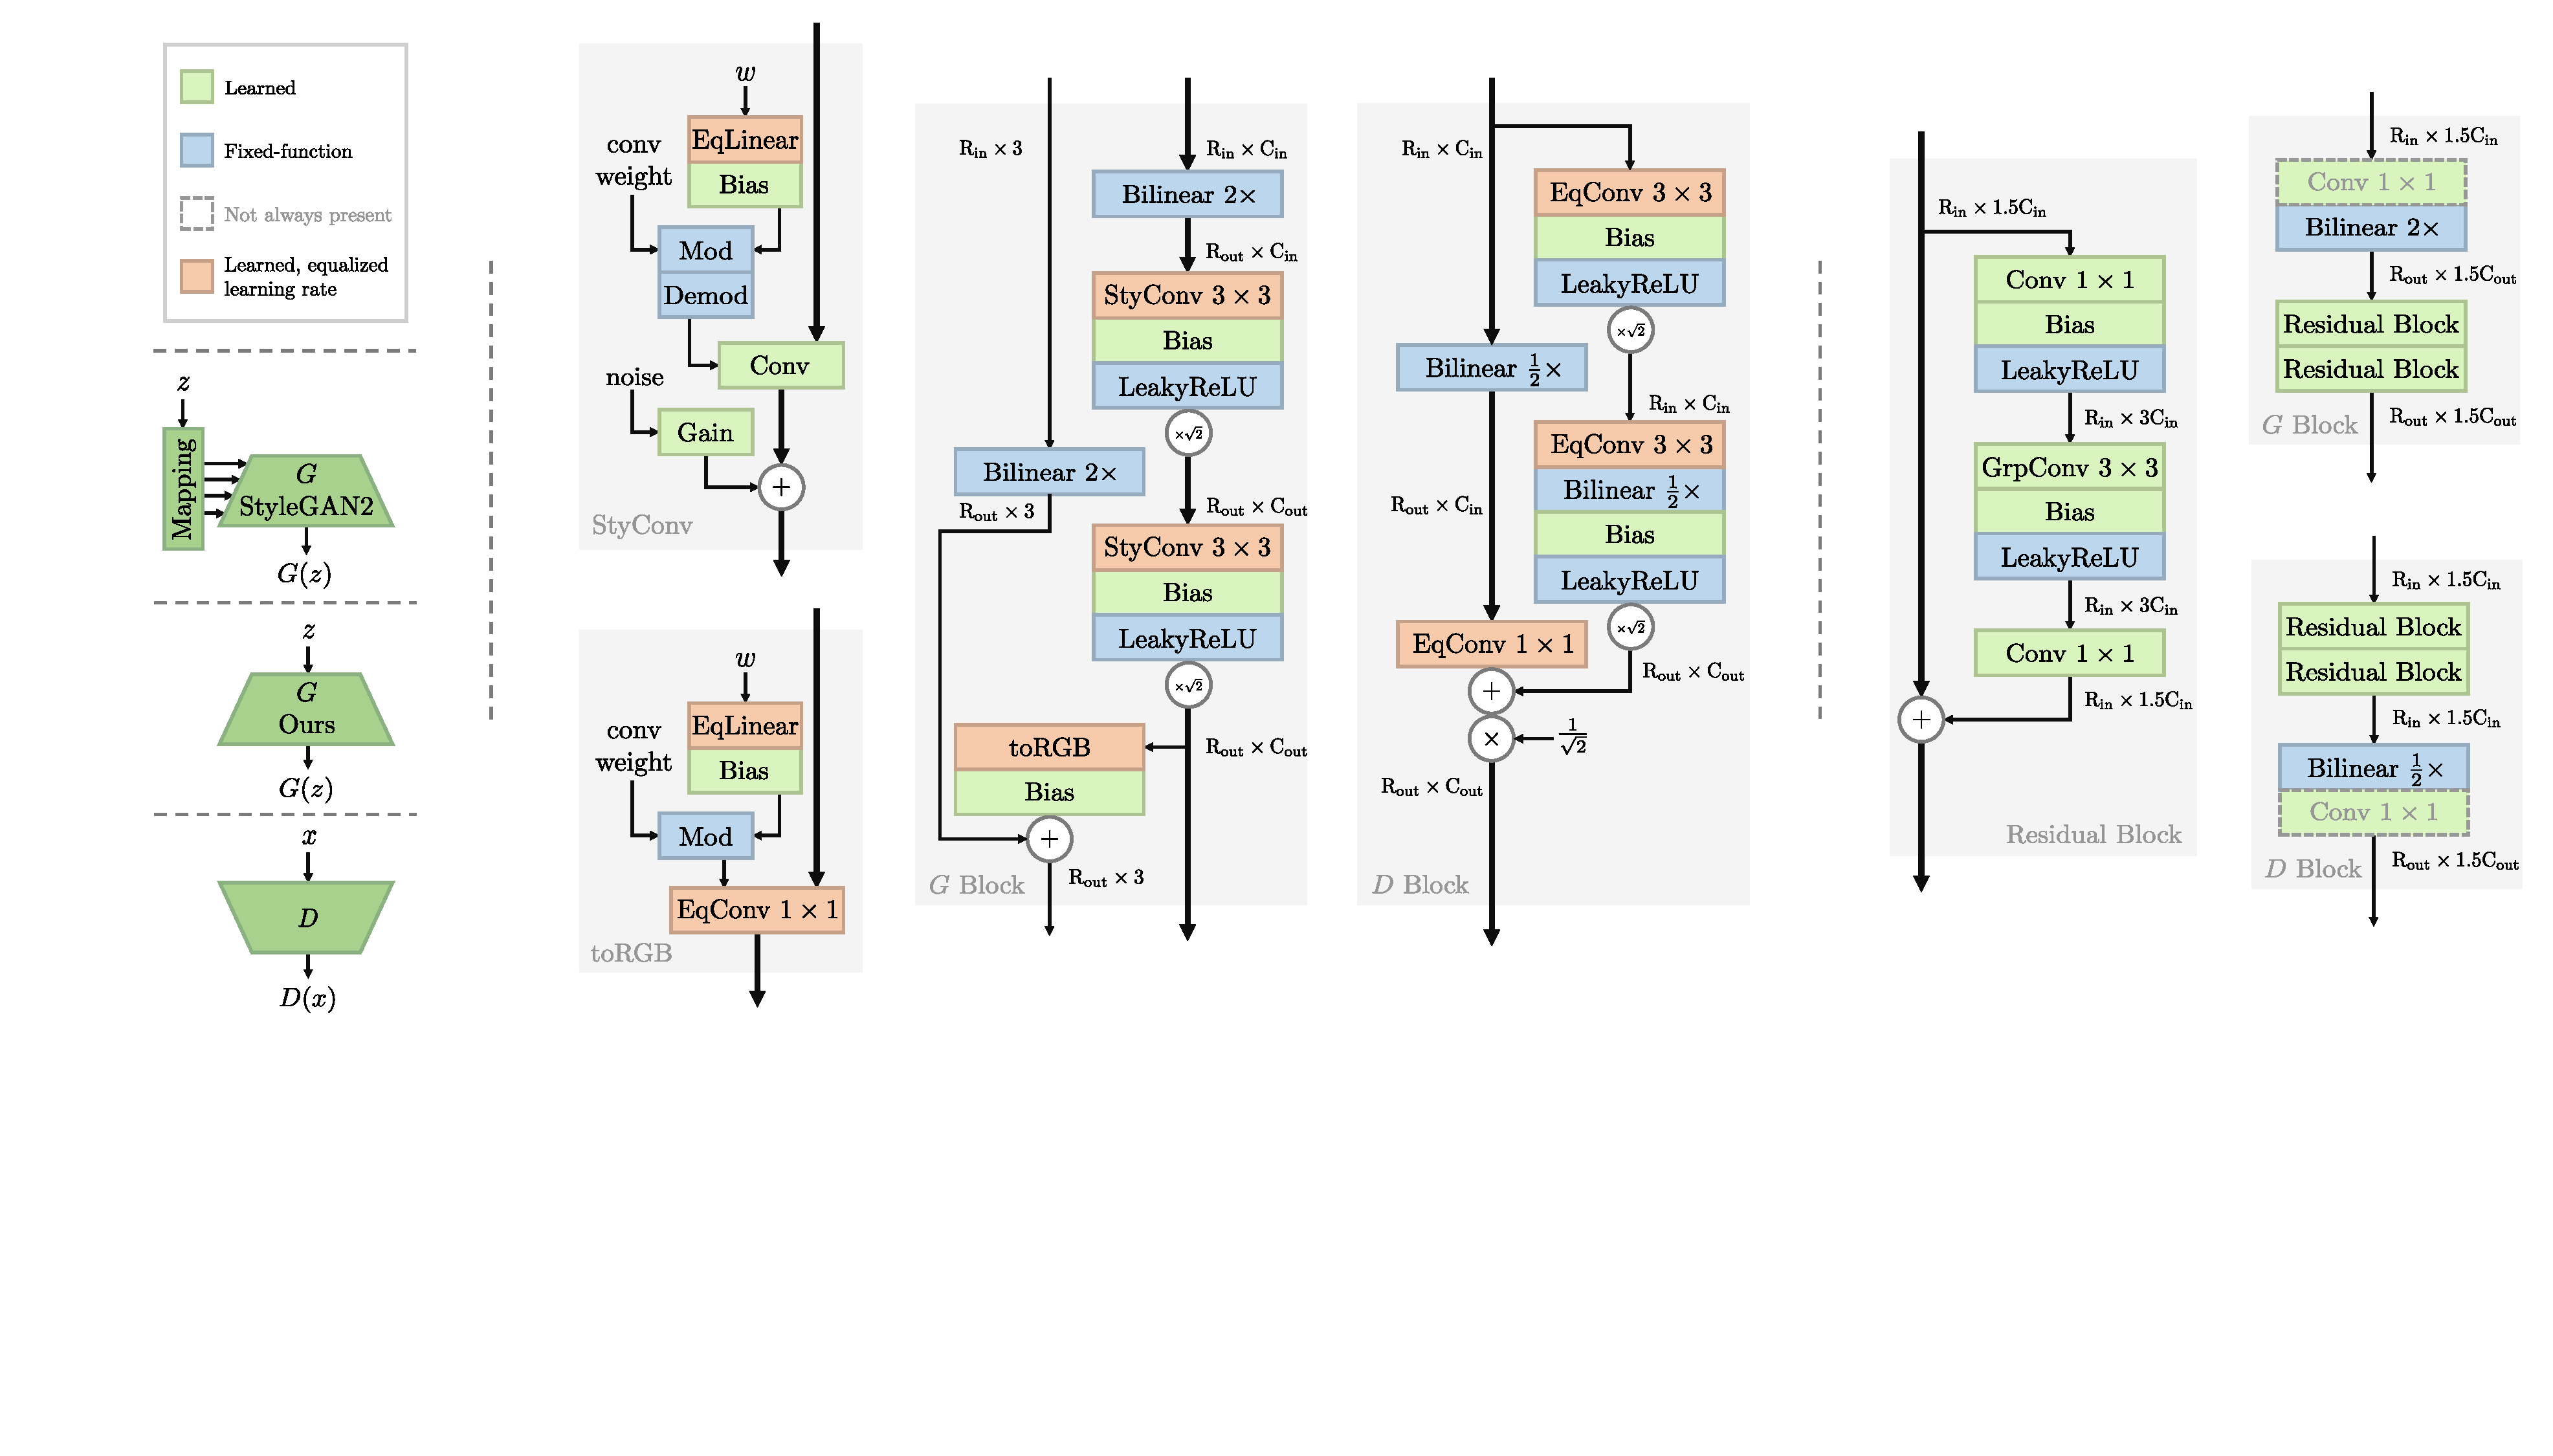
\includegraphics[width=\linewidth,clip,trim={3.5cm 11.5cm 0cm 0cm}]{figures/arch.pdf}
%     \vspace{-0.5cm}
%     \caption{\textbf{Network architecture block comparison to StyleGANv2}. \emph{Left:} High-level architectures. \emph{Middle:} StyleGANv2. \emph{Right:} Our simpler approach. Figure inspired by EDM2~\cite{edm2}.}
%     \label{fig:network}
% \end{figure*}





% \begin{wrapfigure}[16]{r}{8cm}
%     \vspace{-0.5cm}
%     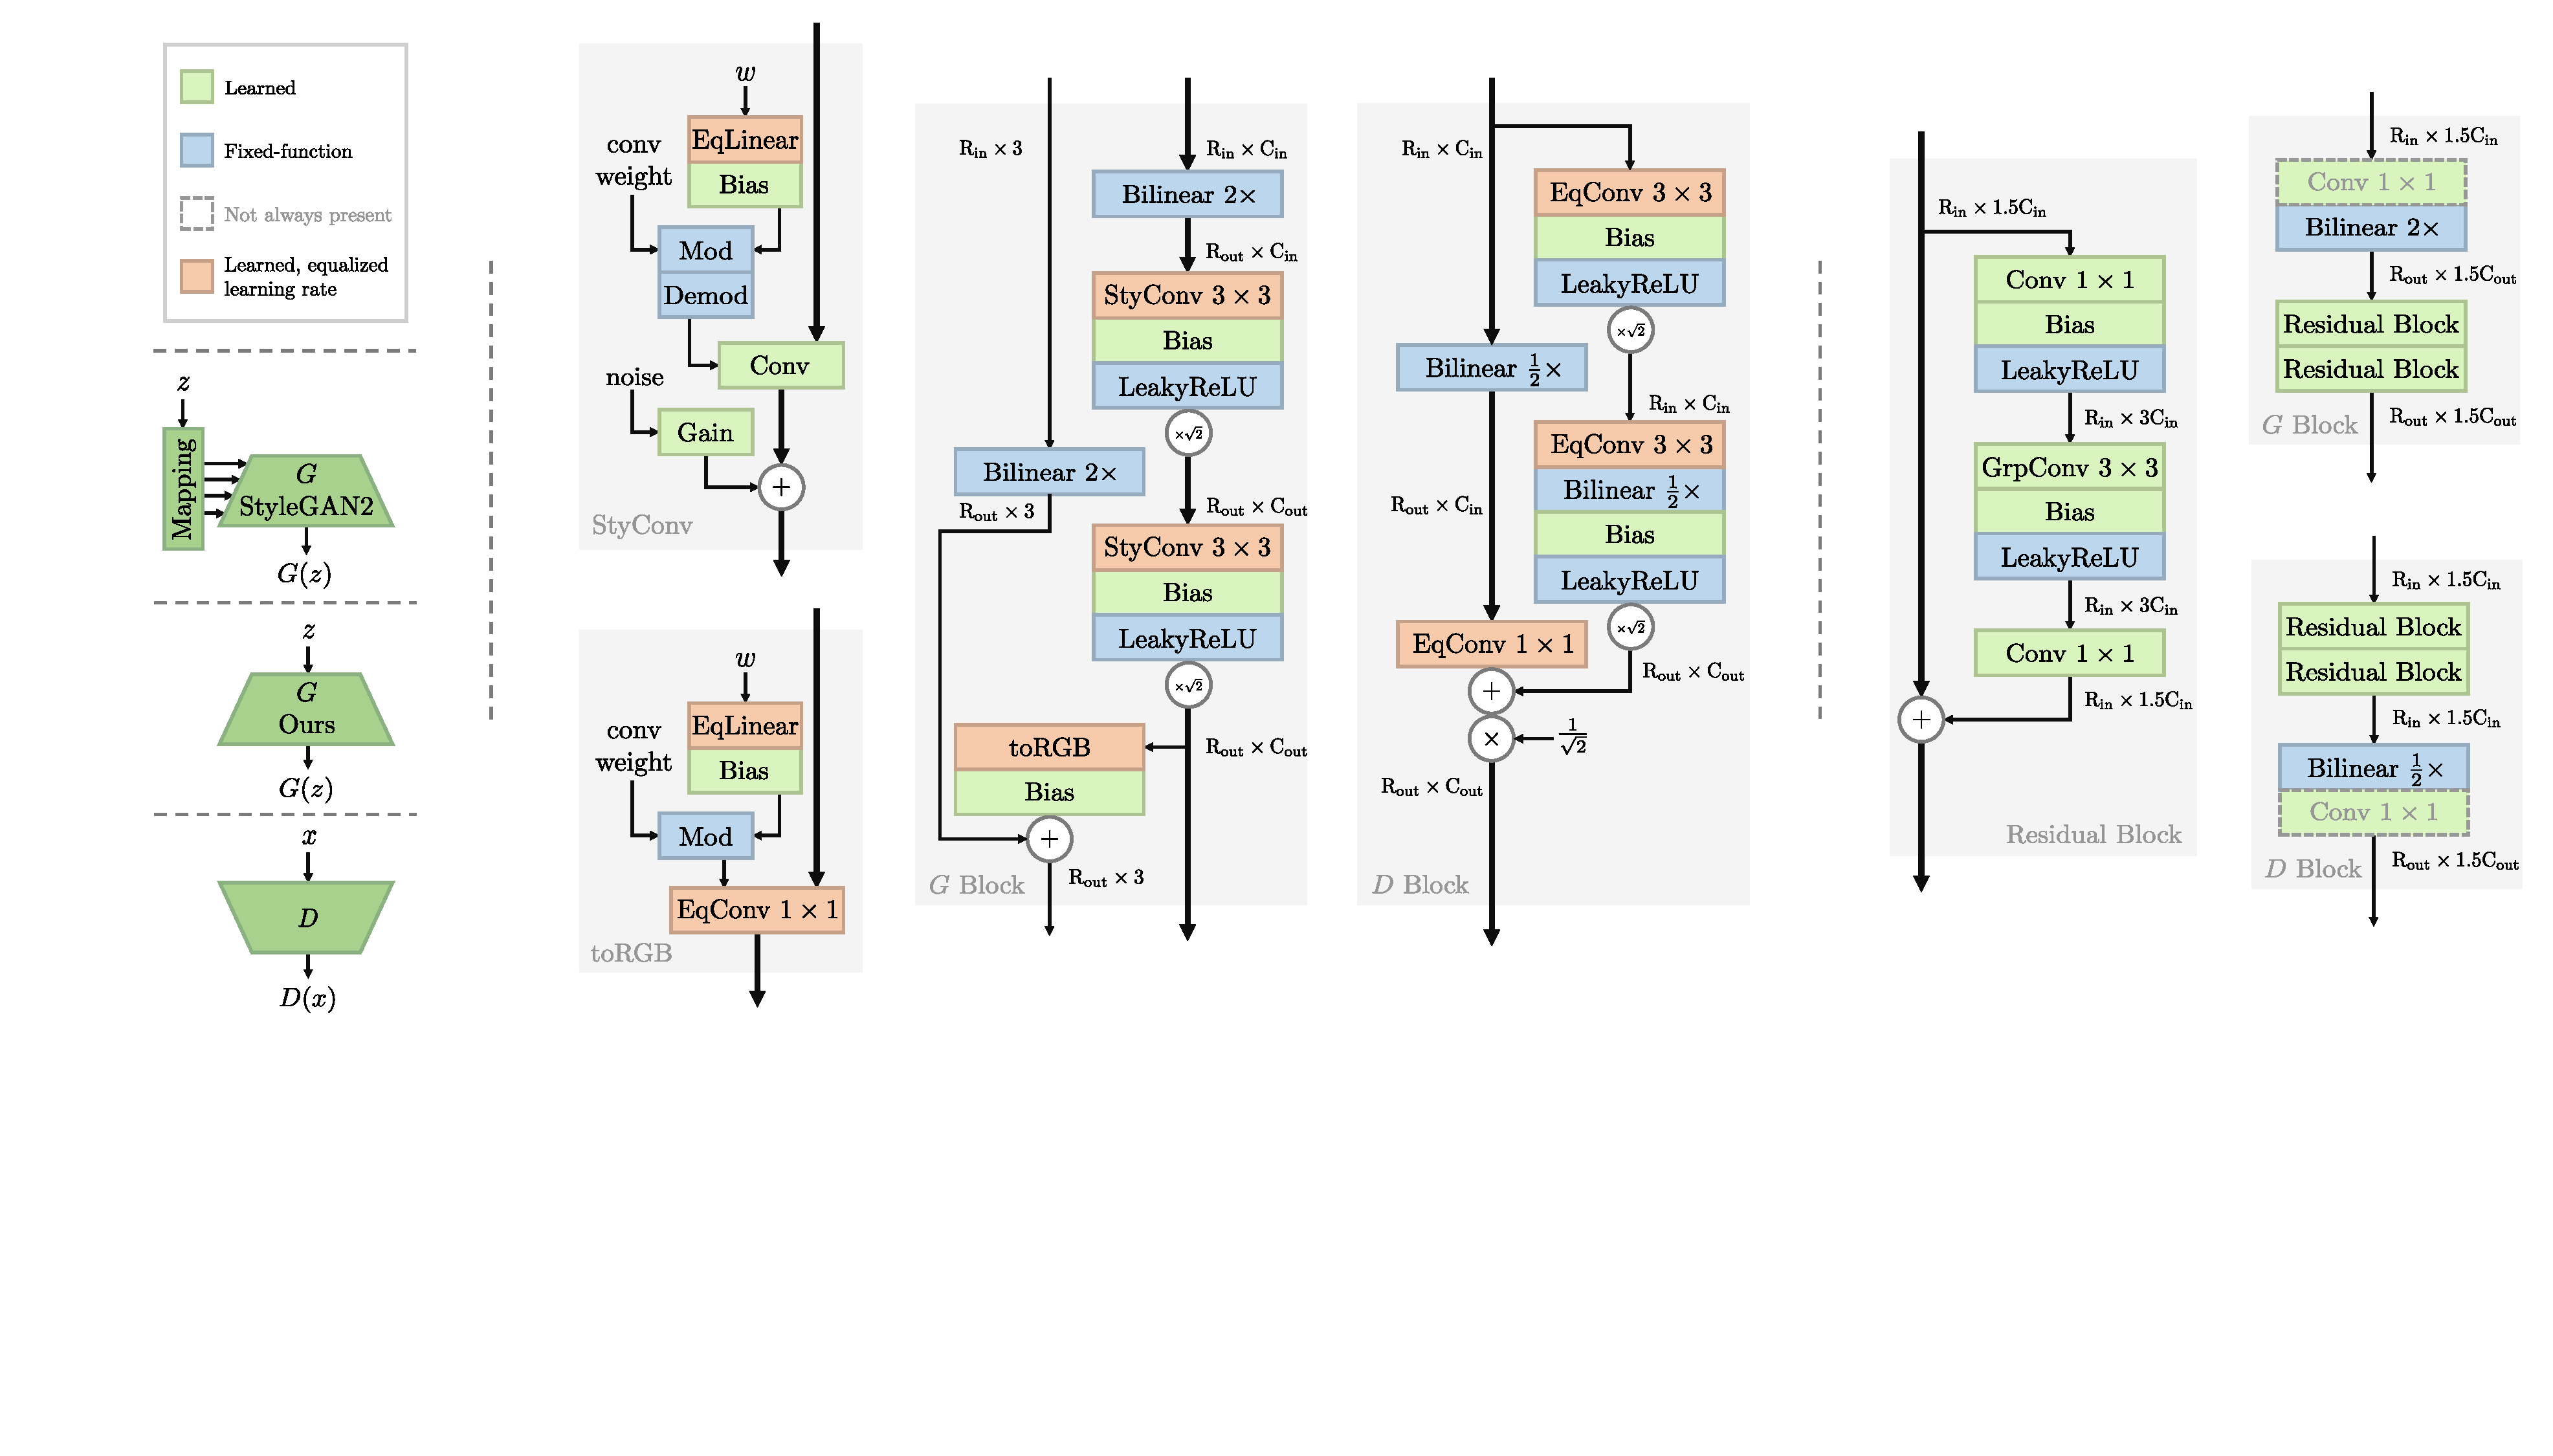
\includegraphics[width=1\linewidth,clip,trim={0cm 0cm 0cm 0cm}]{figures/arch.pdf}
%     \caption{Network architecture blocks.}
%     \label{fig:network}
% \end{wrapfigure}

\paragraph{Bottleneck modernization (Config E).}
Now that we have settled on the overall architecture, we investigate how the residual block can be modernized, specifically i.\ref{item:i1}) and i.\ref{item:i2}). First, we explore i.\ref{item:i1} and replace the 3$\times$3 convolution in the residual block with a grouped convolution. We set the group size to 16 rather than 1 (\ie depthwise convolution as in ConvNeXt) as depthwise convolution is highly inefficient on GPUs and is not much faster than using a larger group size. With grouped convolution, we can reduce the bottleneck compression ratio to two given the same model size. This increases the width of the bottleneck to 1.5$\times$ as wide as Config A. 
%With this, the FID drops to 7.51, surpassing the performance of StyleGAN2. 
Finally, we notice that the compute cost of grouped convolution is negligible compared to 1$\times$1 convolution, and so we seek to enhance the capacity of grouped convolution. We apply i.\ref{item:i2}), which inverts the bottleneck width and the stem width, and which doubles the width of grouped convolutions without any increase in model size. Figure~\ref{fig:network} depicts our final design, which reflects modern CNN architectures.
\vspace{-0.2cm}
\section{Experiments Details}
\label{sec:exp}

\vspace{-0.2cm}
\subsection{Roadmap Insights on FFHQ-256\texorpdfstring{~\cite{sg1}}{}}
\label{sub:arc-experiments}
\vspace{-0.1cm}
As per Table~\ref{tab:roadmap}, Config A (vanilla StyleGAN2) achieves an FID of 7.52 using the official implementation on FFHQ-256. Config B with all tricks removed achieves an FID of 12.46---performance drops as expected. 
Config C, with a well-behaved loss, achieves an FID of 11.65. But, now training is sufficiently stable to improve the architecture.

Config D, which improves $G$ and $D$ based on the classic ResNet and ConvNeXt findings, achieves an FID of 9.95. The output skips of the StyleGAN2 generator are no longer useful given our new architecture; including them produces a worse FID of 10.17. Karras~\etal find that the benefit of output skips is mostly related to gradient magnitude dynamics~\cite{sg3}, and this has been addressed by our ResNet architecture. For StyleGAN2, Karras~\etal conclude that a ResNet architecture is harmful to $G$~\cite{sg2}, but this is not true in our case as their ResNet implementation is considerably different from ours: 1) Karras~\etal use one 3-3 residual block for each resolution stage, while we have a separate transition layer and two 1-3-1 residual blocks; 2) i.3) and i.4) are violated as they do not have a linear residual block~\cite{mobnet} and the transition layer is placed on the skip branch of the residual block rather than the stem; 3) the essential principle of ResNet~\cite{resnet}---identity mapping~\cite{resnet2}---is violated as Karras~\etal divide the output of the residual block by $\sqrt{2}$ to avoid variance explosion due to the absence of a proper initialization scheme.

For Config E, we conduct two experiments that ablate i.\ref{item:i1} (increased width with depthwise conv.) and i.\ref{item:i2} (an inverted bottleneck). We add GroupedConv and reduce the bottleneck compression ratio to two given the same model size. Each bottleneck is now 1.5$\times$ the width of Config A, and the FID drops to 7.51, surpassing the performance of StyleGAN2. By inverting the stem and the bottleneck dimensions to enhance the capacity of GroupedConv, our final model achieves an FID of 7.05, exceeding StyleGAN2.


\begin{wraptable}[12]{r}{6.5cm}
\vspace{-1.25cm}
\centering
\caption{StackedMNIST 1000-mode coverage.}
% Our model outperforms other GANs in terms of $D_\text{KL}$, indicating that we are better able to recover the distribution.}
\vspace{-0.4cm}
\resizebox{0.8\linewidth}{!}{
\begin{tblr}{
  cell{2}{2} = {c},
  cell{2}{3} = {c},
  cell{3}{2} = {c},
  cell{3}{3} = {c},
  cell{4}{2} = {c},
  cell{4}{3} = {c},
  cell{5}{2} = {c},
  cell{5}{3} = {c},
  cell{6}{2} = {c},
  cell{6}{3} = {c},
  cell{7}{2} = {c},
  cell{7}{3} = {c},
  cell{8}{2} = {c},
  cell{8}{3} = {c},
  cell{9}{2} = {c},
  cell{9}{3} = {c},
  cell{10}{2} = {c},
  cell{10}{3} = {c},
  cell{11}{2} = {c},
  cell{11}{3} = {c},
  cell{12}{2} = {c},
  cell{12}{3} = {c},
  hline{2,12} = {1-3}{},
}
Model     & \# modes$\uparrow$ & $D_\text{KL}$$\downarrow$            &  \\
DCGAN~\cite{dcgan}     & 99            & 3.40\phantom{0}&  \\
VEEGAN~\cite{srivastava2017veegan}    & 150           & 2.95\phantom{0}&  \\
WGAN-GP~\cite{wgan-gp}& 959           & 0.73\phantom{0}&  \\
PacGAN~\cite{pacgan}    & 992           & 0.28\phantom{0}&  \\
StyleGAN2~\cite{sg2} & 940           & 0.42\phantom{0}&  \\
PresGAN~\cite{presgan}   & \textbf{1000} & 0.12\phantom{0}&  \\
Adv. DSM~\cite{advsm}  & \textbf{1000} & 1.49\phantom{0}&  \\
VAEBM~\cite{vaebm}     & \textbf{1000} & 0.087          &  \\
DDGAN~\cite{ddgan}     & \textbf{1000} & 0.071          &  \\
MEG~\cite{meg}       & \textbf{1000} & 0.031          &  \\
Ours---Config E     & \textbf{1000} & \textbf{0.029} &  
\end{tblr}
}
\label{tab:stackedmnist}
\end{wraptable}%

\subsection{Mode Recovery --- StackedMNIST\texorpdfstring{~\cite{metz2016unrolled}}{}} 
\vspace{-0.1cm}
We repeat the earlier experiment in 1000-mode convergence on StackedMNIST (unconditional generation), but this time with our updated architecture and with comparisons to SOTA GANs and likelihood-based methods (Tab.~\ref{tab:stackedmnist}, Fig.~\ref{fig:stacked-mnist}). 
One advantage brought up of likelihood-based models such as diffusion over GANs is that they achieve mode coverage~\cite{adm}. We find that most GANs struggle to find all modes. But, PresGAN~\cite{presgan}, DDGAN~\cite{ddgan}, and our approach are successful. Further, our method outperforms all other tested GAN models in term of KL divergence.

\subsection{FID --- FFHQ-256\texorpdfstring{~\cite{sg1}}{} (Optimized)}
\vspace{-0.1cm}
We train Config E model until convergence and with optimized hyperparameters and training schedule on FFHQ at 256$\times$256 (unconditional generation) (Tab.~\ref{tab:ffhq256}, Figs.~\ref{fig:ffhq-256-teaser} and~\ref{fig:ffhq-256}). 
Please see our supplemental material for training details.
%The hyperparameters and schedule are listed in the supplemental material. 
Our model outperforms existing StyleGAN methods, plus four more recent diffusion-based methods. On this common dataset experimental setting, many methods (not listed here) use the bCR~\cite{zhao2021improved} trick---this has only been shown to improve performance on FFHQ-256 (not even at different resolutions of FFHQ)~\cite{zhao2021improved, zhang2022styleswin}. We do not use this trick. 
% no such tricks in our method.
% JT Try to minimize embellishment...
% This is particularly impressive given the fact that the dataset FFHQ was designed for StyleGAN~\cite{sg1} and the StyleGAN series of models were optimized with this specific dataset in mind.
% to achieve this performance.

\subsection{FID --- FFHQ-64\texorpdfstring{~\cite{edm}}{}}
\vspace{-0.1cm}
To compare with EDM~\cite{edm} directly, we evaluate our model on FFHQ at 64$\times$64 resolution. For this, we remove the two highest resolution stages of our 256$\times$256 model, resulting in a generator that is less than half the number of parameters as EDM. Despite this, our model outperforms EDM on this dataset and needs one function evaluation only (Tab.~\ref{tab:ffhq64}).

\begin{figure}
\begin{floatrow}
    %\hspace{-0.75cm}%
    \capbtabbox{%
        \centering
        \resizebox{\linewidth}{!}{
        \begin{tblr}{
          column{2,3} = {r},
          cell{1}{2} = {c},
          cell{1}{3} = {c},
          hline{2,5,9,10} = {-}{},
        }
        Model       & NFE$\downarrow$ & FID$\downarrow$  \\
        StyleGAN2~\cite{sg2}   & 1               & 3.78 \\
        StyleGAN3-T~\cite{sg3} & 1               & 4.81 \\
        StyleGAN3-R~\cite{sg3} & 1               & 3.92 \\
        LDM~\cite{rombach2022high} & 200               & 4.98\\
        ADM (DDIM)~\cite{adm,compdiff} & 500               & 8.41\\
        ADM (DPM-Solver)~\cite{adm,compdiff} & 500               & 8.40\\
        Diffusion Autoencoder~\cite{diffae,compdiff} & 500               & 5.81\\
        Ours---Config E  & 1               & 2.75 \\
        \emph{With ImageNet feature leakage~\cite{kynkaanniemi2022role}:} & & \\
        PolyINR*~\cite{singh2023polynomial} & 1               & 2.72 \\
        StyleGAN-XL*~\cite{sgxl} & 1               & 2.19 \\
        StyleSAN-XL*~\cite{takida2024san} & 1               & 1.68 \\
        \end{tblr}
        }
    }{%
        \caption{
        \label{tab:ffhq256}FFHQ-256. * denotes models that leak ImageNet features.}
    }
    %
    \capbtabbox{%
        \centering
        \resizebox{0.85\linewidth}{!}{
        \begin{tblr}{
          column{2} = {r},
          column{3} = {r},
          hline{2,5,8} = {-}{},
        }
        Model         & NFE$\downarrow$ & FID$\downarrow$ \\
        StyleGAN2~\cite{sg2,anycostgan}     & 1               & 3.32            \\
        MSG-GAN~\cite{karnewar2020msg,anycostgan}       & 1               & 2.7             \\
        Anycost GAN~\cite{anycostgan}   & 1               & 2.52            \\
        VE~\cite{sde,edm}            & 79              & 25.95           \\
        VP~\cite{sde,edm}            & 79              & 3.39            \\
        EDM~\cite{edm}           & 79              & 2.39            \\
        Ours—Config E & 1               & 1.95 \\
        \end{tblr}
        }
    }{%
        \caption{\label{tab:ffhq64}FFHQ-64.}
    }
\end{floatrow}
\vspace{-0.25cm}
\end{figure}


% \begin{figure}
% \begin{floatrow}
%     \capbtabbox{%
%         \centering
%         \resizebox{0.8\linewidth}{!}{
%         \begin{tblr}{
%           column{2,3} = {r},
%           cell{1}{2} = {c},
%           cell{1}{3} = {c},
%           hline{2,9,13} = {-}{},
%         }
%         Model               & NFE$\downarrow$ & FID$\downarrow$ \\
%         BigGAN~\cite{biggan}              & 1               & 14.73 \\
%         TransGAN~\cite{trans}            & 1               & 9.26 \\
%         ViTGAN~\cite{vitgan}              & 1               & 6.66 \\
%         DDGAN~\cite{ddgan}               & 4               & 3.75 \\
%         Diffusion StyleGAN2~\cite{diffusiongan} & 1               & 3.19 \\
%         StyleGAN2 + ADA~\cite{sg2ada}     & 1               & 2.42 \\
%         StyleGAN3-R + ADA~\cite{sg3,studio}   & 1               & 10.83 \\
%         DDPM~\cite{ddpm}               & 1000            & 3.21 \\
%         DDIM~\cite{ddim}                & 50             & 4.67 \\
%         VE~\cite{sde,edm}                  & 35              & 3.11 \\
%         VP~\cite{sde,edm}                  & 35              & 2.48 \\
%         Ours---Config E     & 1               & 1.96 \\
%         \hline
%         \emph{With ImageNet feature leakage~\cite{kynkaanniemi2022role}:} & & \\
%         StyleGAN-XL*~\cite{sgxl}       & 1               & 1.85 \\
%         \end{tblr}
%         }
%     }{%
%         \caption{\label{tab:cifar10}CIFAR-10.}
%     }
%         % \begin{tblr}{
%         %   column{2,3} = {r},
%         %   cell{1}{2}{3} = {},
%         %   hline{2,9,13} = {-}{},
%         % }
%         % Model               & FID$\downarrow$ & Params          \\
%         % BigGAN~\cite{biggan}              & 14.73  & --       \\
%         % TransGAN~\cite{trans}            & 9.26 & --         \\
%         % ViTGAN~\cite{vitgan}              & 6.66 & --         \\
%         % DDGAN~\cite{ddgan}               & 3.75 & --         \\
%         % Diffusion StyleGAN2 & 3.19 & 40.1M           \\
%         % StyleGAN2 + ADA     & 2.42 & 40.1M          \\
%         % StyleGAN3-R + ADA   & 10.83 & 40.1M        \\
%         % DDPM               & 3.21 & 35.2M         \\
%         % DDIM                & 4.67 & --         \\
%         % VE~\cite{edm}                  & 3.11 & 61.8M        \\
%         % VP~\cite{edm}                  & 2.48 & 61.8M         \\
%         % Ours---Config E     & \textbf{1.99}  & 43.0M \\
%         % StyleGAN-XL*~\cite{sgxl}       & 	1.85 & 140.0M \\
%         % \end{tblr}
        
%     %     }
%     % }{%
%     %     \caption{\label{tab:cifar10}CIFAR-10.}
%     % }%
%     %\hspace{-0.75cm}%
%     %\hspace{-0.5cm}%
% \end{floatrow}
% \end{figure}

\subsection{FID --- CIFAR-10~\cite{krizhevsky2009learning}} \vspace{-0.1cm}

\begin{wraptable}[14]{r}{6.5cm}
\vspace{-0.75cm}
\centering
\caption{\label{tab:cifar10}CIFAR-10 performance.}
\vspace{-0.4cm}
\resizebox{0.9\linewidth}{!}{
    \begin{tblr}{
          column{2,3} = {r},
          cell{1}{2} = {c},
          cell{1}{3} = {c},
          hline{2,9,13} = {-}{},
        }
        Model               & NFE$\downarrow$ & FID$\downarrow$ \\
        BigGAN~\cite{biggan}              & 1               & 14.73 \\
        TransGAN~\cite{trans}            & 1               & 9.26 \\
        ViTGAN~\cite{vitgan}              & 1               & 6.66 \\
        DDGAN~\cite{ddgan}               & 4               & 3.75 \\
        Diffusion StyleGAN2~\cite{diffusiongan} & 1               & 3.19 \\
        StyleGAN2 + ADA~\cite{sg2ada}     & 1               & 2.42 \\
        StyleGAN3-R + ADA~\cite{sg3,studio}   & 1               & 10.83 \\
        DDPM~\cite{ddpm}               & 1000            & 3.21 \\
        DDIM~\cite{ddim}                & 50             & 4.67 \\
        VE~\cite{sde,edm}                  & 35              & 3.11 \\
        VP~\cite{sde,edm}                  & 35              & 2.48 \\
        Ours---Config E     & 1               & 1.96 \\
        \hline
        \emph{With ImageNet feature leakage~\cite{kynkaanniemi2022role}:} & & \\
        StyleGAN-XL*~\cite{sgxl}       & 1               & 1.85 \\
        \end{tblr}
}
\end{wraptable}

We train Config E model until convergence and with optimized hyperparameters and training schedule on CIFAR-10 (conditional generation) (Tab.~\ref{tab:cifar10}, Fig.~\ref{fig:cifar10}). Our method outperforms many other GANs by FID even though the model has relatively small capacity. For instance, StyleGAN-XL~\cite{sgxl} has 18\ M parameters in the generator and 125\ M parameters in the discriminator, while our model has a 40\ M parameters between the generator and discriminator combined (Fig.~\ref{fig:fid-50k-vs-params-cifar-10}). Compared to diffusion models like LDM or ADM, GAN inference is significantly cheaper as it requires only one network function evaluation compared to the tens or hundreds of network function evaluations for diffusion models without distillation. 

\begin{wrapfigure}[12]{r}{6.5cm}
    \vspace{-0.4cm}
    \centering
    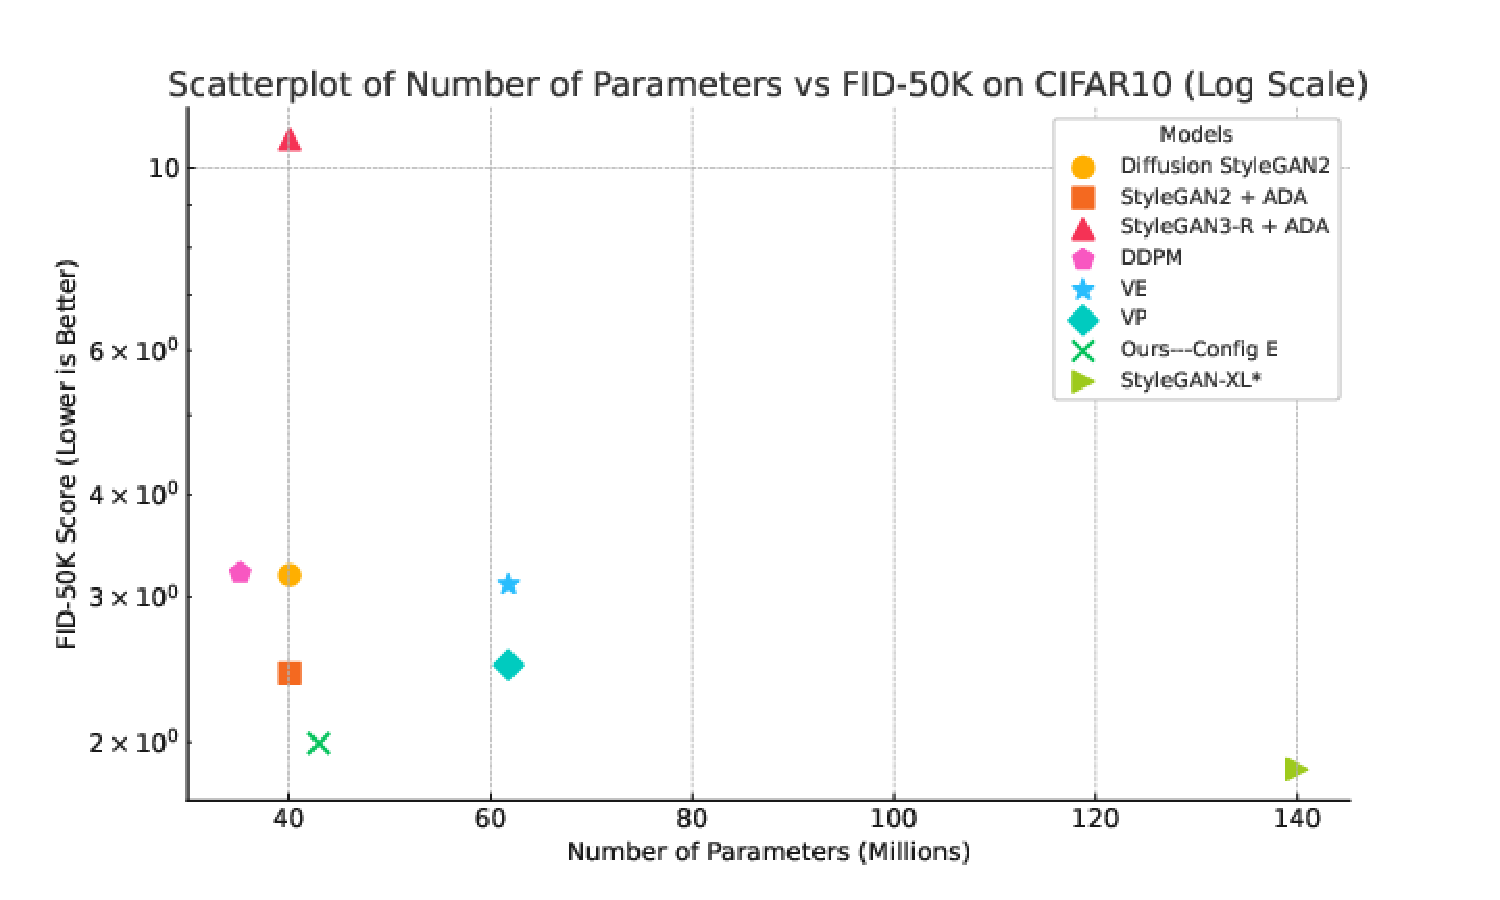
\includegraphics[width=\linewidth,clip,trim={0 0 0 2cm}]{figures/Scatterplot-FID-Parameters-CIFAR10.pdf}
    \caption{Millions of parameters vs.~FID-50K (log scale) on CIFAR-10. Lower is better.}
    \label{fig:fid-50k-vs-params-cifar-10}
\end{wrapfigure}

Many state-of-the-art GANs are derived from Projected GAN~\cite{sauer2021projected}, including StyleGAN-XL~\cite{sgxl} and the concurrent work of StyleSAN-XL~\cite{takida2024san}. These methods use a pre-trained ImageNet classifier in the discriminator. Prior work has shown that a pre-trained ImageNet discriminator can leak ImageNet features into the model~\cite{kynkaanniemi2022role}, causing the model to perform better when evaluating on FID since it relies on a pre-trained ImageNet classifier for the loss. But, this does not improve results in perceptual studies~\cite{kynkaanniemi2022role}. Our model produces its low FID without any ImageNet pre-training.

%\jt{Missing citations here for such methods.}


%\aaron{add NFEs}
%\jt{Which models in our evaluation use this? Any?}

%\jt{What is the second caveat?}

\subsection{FID --- ImageNet-32~\cite{chrabaszcz2017downsampled}}
\label{sec:imagenet32-fid-explain}
We train Config E model until convergence and with optimized hyperparameters and training schedule on ImageNet-32 (conditional generation). We compare against recent GAN models and recent diffusion models in Table~\ref{tab:imagenet32}.
We adjust the number of parameters in the generator of our model to match StyleGAN-XL~\cite{sgxl}'s generator (84M parameters). Specifically, we make the model significantly wider to match. Our method achieves comparable FID despite using a 60\% smaller discriminator (Tab.~\ref{tab:imagenet32}) and despite not using a pre-trained ImageNet classifier.
%, which has been shown to improve FID performance, but not improve results in perceptual studies~\cite{kynkaanniemi2022role}.

\vspace{-0.1cm}
\subsection{FID --- ImageNet-64~\cite{chrabaszcz2017downsampled}}
We evaluate our model on ImageNet-64 to test its scalability. We stack another resolution stage on our ImageNet-32 model, resulting in a generator of 104\ M parameters. This model is nearly 3$\times$ smaller than diffusion-like models~\cite{adm,edm,cm,icm} that rely on the ADM backbone, which contains about 300\ M parameters. Despite the smaller model size and that our model generates samples in one step, it outperforms larger diffusion models with many NFEs on FID (Tab.~\ref{tab:imagenet64}).

\vspace{-0.1cm}
\subsection{Recall}
We evaluate the recall~\cite{precrecall} of our model on each dataset to quantify sample diversity. In general, our model achieves a recall that is similar to or marginally worse than the diffusion model counterpart, yet superior to existing GAN models. For CIFAR-10, the recall of our model peaked at 0.57; as a point of comparison, StyleGAN-XL~\cite{sgxl} has a worse recall of 0.47 despite its lower FID. For FFHQ, we obtain a recall of 0.53 at 64$\times$64 and 0.49 at 256$\times$256, whereas StyleGAN2~\cite{sg2} achieved a recall of 0.43 on FFHQ-256. Our ImageNet-32 model achieved a recall of 0.63; comparable to ADM~\cite{adm}. Our ImageNet-64 model achieved recall 0.59. While this is slightly worse than $\approx$0.63 that many diffusion models achieve, it is better than BigGAN-deep~\cite{biggan} which achieved a recall of 0.48.

\begin{figure}
    \begin{floatrow}
        \capbtabbox{%
        \centering
        \resizebox{0.9\linewidth}{!}{
        \begin{tblr}{
          column{2} = {r},
          column{3} = {r},
          cell{8}{1} = {c=3}{},
          hline{2,7-8} = {-}{},
        }
    Model                                                       & NFE$\downarrow$  & FID$\downarrow$                        \\ 
    DDPM++~\cite{kim2021soft}                  & 1000 & 8.42                                   \\
    VDM~\cite{kingma2021variational}           & 1000 & 7.41                                   \\
    MSGAN~\cite{karnewar2020msg,ning2023input} & 1    & 12.3                                   \\
    ADM~\cite{adm}                             & 1000 & 3.60                                   \\
    DDPM-IP~\cite{ning2023input}               & 1000 & 2.87                                   \\
    Ours—Config E               & 1    & 1.27   \\
    \textit{With ImageNet feature leakage~\cite{kynkaanniemi2022role}:}    \\
    StyleGAN-XL*~\cite{sgxl}                   & 1    & 1.10                                  
    \end{tblr}
        }
    }{%
        \caption{\label{tab:imagenet32}ImageNet-32.}
        % \jt{some are conditional still}}
    }
    %
    \capbtabbox{
        \centering
        \resizebox{0.9\linewidth}{!}{
        \begin{tblr}{
          column{2} = {r},
          column{3} = {r},
          cell{1}{2} = {c},
          cell{1}{3} = {c},
          cell{12}{1} = {c=3}{},
          hline{2-3,11-12} = {-}{},
        }
        Model         & NFE$\downarrow$ & FID$\downarrow$ \\
        BigGAN-deep~\cite{biggan}\phantom{xx}   & 1               & 4.06            \\
        DDPM~\cite{ddpm}          & 250             & 11.0            \\
        DDIM~\cite{ddim}          & 50              & 13.7            \\
        ADM~\cite{adm}           & $^\S$250             & 2.91            \\
        EDM~\cite{edm}           & 79              & 2.23            \\
        CT~\cite{cm}            & 2               & 11.1            \\
        CD~\cite{cm}            & 3               & 4.32            \\
        iCT-deep~\cite{icm}      & 2               & 2.77            \\
        DMD~\cite{dmd}           & 1               & 2.62            \\
        Ours—Config E & 1               & 2.09            \\
        \emph{With ImageNet feature leakage~\cite{kynkaanniemi2022role}:}          &                 &                 \\
        StyleGAN-XL*~\cite{sgxl}   & 1               & 1.52            
        \end{tblr}
        }
    }
    {
        \caption{\label{tab:imagenet64}ImageNet-64.\hspace{-0.1cm} {\small \S:\hspace{-0.05cm}deterministic sampling.}}
    }
    \end{floatrow}
    \vspace{-0.25cm}
\end{figure}


% \begin{table}[ht]
%     \centering
%     \begin{tabular}{lcccccccc}
%         \toprule
%         \textbf{Model} & \textbf{\# Param.} & \textbf{IS $\uparrow$} & \textbf{FID $\downarrow$} & \textbf{Precision $\uparrow$} & \textbf{Recall $\uparrow$} & \textbf{Density $\uparrow$} & \textbf{Coverage $\uparrow$} & \textbf{Inf. (s)} \\
%         \midrule
%         ReACGAN + DiffAug (Ours) [10] & 9.4M & 10.15 & 2.64 & 0.75 & 0.65 & 0.98 & 0.90 & 0.009 \\
%         StyleGAN2-ADA [85] & 20.2M & 10.31 & 2.41 & 0.74 & 0.68 & 1.02 & 0.92 & 0.008 \\
%         StyleGAN2-ADA (Ours) [85] & 20.2M & \textbf{10.53} & 2.31 & 0.75 & 0.69 & 1.04 & 0.93 & 0.008 \\
%         StyleGAN2 + DiffAug + D2D-CE (Ours) [10] & 20.2M & 10.46 & 2.30 & 0.76 & 0.68 & 1.03 & 0.93 & 0.007 \\
%         DDPM [43] & 35.2M & 9.73 & 3.23 & 0.78 & 0.67 & 1.10 & 0.93 & 15.422 \\
%         DDPM++ [44] & 106.6M & 9.90 & 2.49 & 0.78 & 0.69 & 1.12 & 0.94 & 46.697 \\
%         NCSN++ [44] & 107.6M & 10.08 & 2.27 & 0.77 & 0.70 & 1.07 & 0.94 & 99.304 \\
%         LSGM [45] & - & 10.04 & 2.80 & 0.80 & 0.70 & 1.15 & 0.95 & - \\
%         LSGM-ODE [45] & - & 10.07 & \textbf{2.09} & 0.77 & 0.71 & 1.03 & 0.94 & - \\
%         CLD-SGM [47] & - & 9.88 & 2.38 & 0.78 & 0.69 & 1.12 & 0.94 & - \\
%         StyleGAN-XL~ & 18.0M & \textbf{11.03} & \textbf{1.88} & 0.77 & 0.59 & 1.08 & 0.94 & 0.010 \\
%         % BaselineGAN & %10.284011840820312
%         % 10.28
%         % & %1.9925376117527978 
%         % 1.99 & % 0.6899600028991699 
%         % 0.69 &&
%         \bottomrule
%     \end{tabular}
%     \caption{Comparison of various models on CIFAR10 dataset. TODO fix citation}
% \label{tab:cifar10_comparison}
%\end{table}

% \jt{Is the below meant to be a conclusion? Some of these statements are unfounded in the evidence we present so far.}
% \begin{enumerate}

%     \item We demonstrate the ability of our method to recover all modes of training data on Stacked Mnist~\ref{tab:stackedmnist}.
%     \item We beat all methods that do not use bCR (shown to overfit for FFHQ-256~\cite{}) and methods that do not leak imagenet features from a pretrained discriminator~\cite{kynkaanniemi2022role}. If we exclude these two categories of models, we are SOTA across all open source GANs. We also SOTA on a per parameter count basis on multiple GANs.
%     \item We demonstrate SOTA performance on CIFAR-10 image generation at our current parameter count, outperforming all previous GANs except for StyleGAN-XL derived ones with X\% percent of the parameters of these methods. We also do not leak features from ImageNet or use a pretrained discriminator.~\ref{tab:cifar10}. 
%     \item We achieve near SOTA on FFHQ 256 and achieve SOTA for a GAN method without bCR or feature leakage.
%     \item We achieve near state of the art results on Imagenet and achieve Pareto frontier results for total GAN model parameter size.
% \end{enumerate}
% \begin{table}[h]
\centering
\caption{FID on ImageNet-32}
\begin{tabular}{ l c c }
\toprule
Model & \textbf{Year} & FID$\downarrow$ \\
\midrule
% %Real NVP (Dinh et al.) & 2016 & 4.28 \\
% %Glow (Kingma and Dhariwal) & 2018 & 4.09 \\
% %MintNet & 2019 & 4.06 \\
% % Residual Flow & 2019 & 4.01 \\
% % BIVA Maaloe et al. & 2019 & 3.96 \\
% % ANF Huang et al. & 2020 & 3.92 \\
% % NVAE w/ flow & 2020 & 3.92 \\
% % PixelRNN & 2016 & 3.86 \\
% % Flow++ & 2019 & 3.86 \\
% % SPN Menick and Kalchbrenner & 2018 & 3.85 \\
% % Gated PixelCNN & 2016 & 3.83 \\
% % Very Deep VAE & 2020 & 3.8 \\
% % MRCNF & 2021 & 3.77 \\
% % $\delta$-VAE & 2019 & 3.77 \\
% Image Transformer~\cite{parmar2018image} & 2018 & 3.77 \\
% ScoreFlow & 2021 & 3.76 \\
% Reflected Diffusion & 2023 & 3.74 \\
% %Hourglass & 2021 & 3.74 \\
% DenseFlow-74-10 & 2021 & 3.63 \\
% i-DODE & 2023 & 3.43 \\
% MSGAN~\cite{karnewar2020msg} & 2019 & 12.3 \\
% DDPM-IP & 2023 & 2.66 \\
MSGAN~\cite{karnewar2020msg} & 2019 & 12.3 \\
VDM~\cite{kingma2021variational} & 2021 & 7.41 \\
DDPM++~\cite{kim2021soft} & 2021 & 8.42 \\
DDPM-IP~\cite{ning2023input} & 2023 & 2.87 \\
\textbf{Ours} & 2024 & 1.28 \\
StyleGAN-XL~\cite{sauer2022stylegan} & 2022 & \textbf{1.10} \\
\bottomrule
\end{tabular}
\end{table}

% \begin{table}[tO]
%     \centering
%     \begin{tabular}{c|c|c|c}
%          & FID\_50k & Precision & Recall \\
%         StyleGAN &  \\
%         StyleGAN-XL? &
%         Lots of other baselines
%     \end{tabular}
%     \caption{Caption}
%     \label{tab:my_label}
% \end{table}
% \label{sec:exp}
% % cifar10, ffhq, imagenet

% \begin{table}
%     \centering
%     %\caption{Results for CIFAR-10 generation. \aaron{add NFEs}}
%     %\vspace{-2mm}
%     \begin{tblr}{
%       column{2} = {r},
%       cell{1}{2} = {c},
%       hline{2,9,13} = {-}{},
%     }
%     Model               & FID$\downarrow$           \\
%     BigGAN~\cite{biggan}              & 14.73         \\
%     TransGAN~\cite{trans}            & 9.26          \\
%     ViTGAN~\cite{vitgan}              & 6.66          \\
%     DDGAN~\cite{ddgan}               & 3.75          \\
%     Diffusion StyleGAN2 & 3.19          \\
%     StyleGAN2 + ADA     & 2.42          \\
%     StyleGAN3-R + ADA   & 10.83         \\
%     DDPM                & 3.21          \\
%     DDIM                & 4.67          \\
%     VE                  & 3.11          \\
%     VP                  & 2.48          \\
%     Ours---Config E     & \textbf{1.99} 
%     \end{tblr}
%     %\label{tab:cifar10}
%     \caption{Results for CIFAR-10 generation. \aaron{add NFEs}}
%     \label{tab:cifar10}
% \end{table}



%%%%%%%%%%%%%%%%%%%%%%%%%%%%%%%%%%%%%%%%%%%%%%%%%%%%%%%%%%%%%
% Qualitative figures
%%%%%%%%%%%%%%%%%%%%%%%%%%%%%%%%%%%%%%%%%%%%%%%%%%%%%%%%%%%%%

% Variable to control the size of each image
% \begin{figure}
%     \centering
%     \includegraphics{example-image-a}
%     \caption{stacked mnist (qualitative figure) (from powerpoint)}
%     \label{fig:stacked-mnist}
% \end{figure}
% cifar10, ffhq, imagenet

% \noindent\begin{minipage}{.33\textwidth}
% \centering
% \captionof{table}{1000-mode coverage on StackedMNIST.}
% \vspace{-2mm}
% \begin{tblr}{
%   cell{2}{2} = {c},
%   cell{2}{3} = {c},
%   cell{3}{2} = {c},
%   cell{3}{3} = {c},
%   cell{4}{2} = {c},
%   cell{4}{3} = {c},
%   cell{5}{2} = {c},
%   cell{5}{3} = {c},
%   cell{6}{2} = {c},
%   cell{6}{3} = {c},
%   cell{7}{2} = {c},
%   cell{7}{3} = {c},
%   cell{8}{2} = {c},
%   cell{8}{3} = {c},
%   cell{9}{2} = {c},
%   cell{9}{3} = {c},
%   cell{10}{2} = {c},
%   cell{10}{3} = {c},
%   cell{11}{2} = {c},
%   cell{11}{3} = {c},
%   hline{2,11} = {1-3}{},
% }
% Model     & Modes$\uparrow$ & KLD$\downarrow$            &  \\
% DCGAN     & 99            & 3.40\phantom{0}&  \\f
% VEEGAN    & 150           & 2.95\phantom{0}&  \\
% WGAN-GP   & 959           & 0.73\phantom{0}&  \\
% PacGAN    & 992           & 0.28\phantom{0}&  \\
% StyleGAN2 & 940           & 0.42\phantom{0}&  \\
% PresGAN   & \textbf{1000} & 0.12\phantom{0}&  \\
% Adv. DSM  & \textbf{1000} & 1.49\phantom{0}&  \\
% VAEBM     & \textbf{1000} & 0.087          &  \\
% DDGAN     & \textbf{1000} & 0.071          &  \\
% Ours      & \textbf{1000} & \textbf{???} &  
% \end{tblr}
% \label{tab:stackedmnist}
% \end{minipage}%
% \begin{minipage}{.33\textwidth}
% \centering
% \captionof{table}{Results for CIFAR-10 generation.}
% \vspace{-2mm}
% \begin{tblr}{
%   column{2} = {r},
%   cell{1}{2} = {c},
%   hline{2,9,13} = {-}{},
% }
% Model               & FID$\downarrow$           \\
% BigGAN              & 14.73         \\
% TransGAN            & 9.26          \\
% ViTGAN              & 6.66          \\
% DDGAN               & 3.75          \\
% Diffusion StyleGAN2 & 3.19          \\
% StyleGAN2 + ADA     & 2.42          \\
% StyleGAN3-R + ADA   & 10.83         \\
% DDPM                & 3.21          \\
% DDIM                & 4.67          \\
% VE                  & 3.11          \\
% VP                  & 2.48          \\
% Ours                & \textbf{1.99} 
% \end{tblr}
% \label{tab:cifar10}
% \end{minipage}%
% \begin{minipage}{.33\textwidth}
% \centering
% \captionof{table}{Results on FFHQ ($256\times256$).}
% \vspace{-2mm}
% \begin{tblr}{
%   column{2} = {r},
%   cell{1}{2} = {c},
%   hline{2,5} = {-}{},
%   hline{2,9} = {-}{},
% }
% Model       & FID$\downarrow$  \\
% StyleGAN2   & 3.78 \\
% StyleGAN3-T & 4.81 \\
% StyleGAN3-R & 3.92 \\
% LDM & 4.98\\
% ADM (DDIM) & 8.41\\
% ADM (DPM-Solver) & 8.40\\
% Diffusion Autoencoder & 5.81\\
% Ours        & \textbf{2.95} 
% \end{tblr}
% \label{tab:ffhq256}
% \end{minipage}


% \input{tables/cifar10}
% \input{tables/ffhq256}
% \input{tables/MNIST}
\begin{figure}[h!]
    \newlength{\imgsize}
    \setlength{\imgsize}{0.10\linewidth} % Adjust this value to change the size of the images
    
    % New command to include images from a specific directory
    \newcommand{\qualitativeimg}[1]{%
        \includegraphics[width=\imgsize]{figures/qualitative/ffhq-256-000139623/image-#1.jpg}%
    }
    
    \setlength{\tabcolsep}{0pt} % Remove spacing between columns
    \renewcommand{\arraystretch}{0} % Remove spacing between rows
    
    \centering
    \begin{tabular}{cccccccc} % Eight columns
        \qualitativeimg{64} & \qualitativeimg{65} & \qualitativeimg{66} & \qualitativeimg{67} & \qualitativeimg{128} & \qualitativeimg{69} & \qualitativeimg{70} & \qualitativeimg{71} \\
        \qualitativeimg{72} & \qualitativeimg{73} & \qualitativeimg{74} & \qualitativeimg{75} & \qualitativeimg{76} & \qualitativeimg{77} & \qualitativeimg{78} & \qualitativeimg{79} \\
        \qualitativeimg{80} & \qualitativeimg{81} & \qualitativeimg{82} & \qualitativeimg{83} & \qualitativeimg{84} & \qualitativeimg{85} & \qualitativeimg{86} & \qualitativeimg{87} \\
        \qualitativeimg{88} & \qualitativeimg{89} & \qualitativeimg{90} & \qualitativeimg{91} & \qualitativeimg{92} & \qualitativeimg{93} & \qualitativeimg{94} & \qualitativeimg{95} \\
        \qualitativeimg{96} & \qualitativeimg{97} & \qualitativeimg{98} & \qualitativeimg{99} & \qualitativeimg{100} & \qualitativeimg{101} & \qualitativeimg{102} & \qualitativeimg{103} \\
        \qualitativeimg{104} & \qualitativeimg{105} & \qualitativeimg{106} & \qualitativeimg{107} & \qualitativeimg{108} & \qualitativeimg{109} & \qualitativeimg{110} & \qualitativeimg{111} \\
        \qualitativeimg{112} & \qualitativeimg{113} & \qualitativeimg{114} & \qualitativeimg{115} & \qualitativeimg{116} & \qualitativeimg{117} & \qualitativeimg{118} & \qualitativeimg{119} \\
        \qualitativeimg{120} & \qualitativeimg{121} & \qualitativeimg{122} & \qualitativeimg{123} & \qualitativeimg{124} & \qualitativeimg{125} & \qualitativeimg{126} & \qualitativeimg{127} \\
    \end{tabular}
    \caption{Qualitative examples of sample generation from our Config E on FFHQ-256.}
    \label{fig:ffhq-256-teaser}
\end{figure}

\section{Discussion}
\label{sec:discussion}

We discuss related work, limitations, and some future directions.

\paragraph{Related Work.}
\cref{sec:discussion:selection} discusses how the selection mechanism relates to similar concepts.
\cref{sec:related} has an extended related work of SSMs and other related models.

\paragraph{No Free Lunch: Continuous-Discrete Spectrum.}
Structured SSMs were originally defined as discretizations of continuous systems \eqref{eq:ssm},
and have had a strong inductive bias toward continuous-time data modalities such as perceptual signals (e.g.\ audio, video).
As discussed in \cref{sec:method:motivation,sec:method:properties}, the selection mechanism overcomes their weaknesses
on discrete modalities such as text and DNA;
but this conversely can impede their performance on data that LTI SSMs excel on.
Our ablations on audio waveforms examine this tradeoff in more detail.

\paragraph{Downstream Affordances.}
Transformer-based foundation models (particularly LLMs) have a rich ecosystem of properties and modes of interaction with pretrained models,
such as fine-tuning, adaptation, prompting, in-context learning, instruction tuning, RLHF, quantization, and so on.
We are particularly interested in whether Transformer alternatives such as SSMs have similar properties and affordances.

%

\paragraph{Scaling.}
Our empirical evaluation is limited to small model sizes,
below the threshold of most strong open source LLMs (e.g. Llama \citep{touvron2023llama})
as well as other recurrent models such as RWKV~\citep{peng2023rwkv} and RetNet~\citep{sun2023retentive},
which have been evaluated at the 7B parameter scale and beyond.
It remains to assess whether Mamba still compares favorably at these larger sizes.
We also note that scaling SSMs may involve further engineering challenges and adjustments to the model
that are not discussed in this paper.

%



%%%%%%%%% REFERENCES
{\small
\bibliographystyle{ieee_fullname}
\bibliography{bib/face_editing}
}

\appendix
\clearpage
\section*{Appendices}

\section{Implementation}
\label{app:implementation}

% Sampling from a cascade consists of 

\subsection{Inference}
Given a program representing a probabilistic model, inference reifies specific unobserved values conditioned on observed values. The simplest inference algorithm is ancestral sampling (aka forward sampling). The basic inference API is:

\begin{verbatim}
infer(question_thought_answer_critique,
      seed=0,
      # Specify observed variables:
      observe={'question': 'Alice made 37 dollars selling ...',
               'critique': 'The reasoning and arithmetic are correct.'},
      # Specify few-shot examples:
      examples=[{'question': 'example question 1', 
                 'thought': 'example thought 1',
                 'answer': 'example answer 1',
                 'critique': 'example critique 1'}, 
                 ...])
\end{verbatim}

\subsection{Code examples}

In each example below, S is a string distribution. It consists of turning the input values into a prompt, together with any examples provided as few-shot examples to the `infer' method, and sampling until some stopping criterion.

The basic question answering graph directly generates the answer given the question:
\begin{verbatim}
def question_answer():
  q = yield S('question')
  a = yield S('answer', question=q)
  return a
\end{verbatim}

Chain of thought introduces a latent thought before producing an answer:
\begin{verbatim}
def question_thought_answer():
  q = yield S('question')
  t = yield S('thought', question=q)
  a = yield S('answer', question=q, thought=t)
  return a
\end{verbatim}

Self critique introduces a step in which the model critiques its own reasoning in natural language:
\begin{verbatim}
def question_thought_answer_critique():
  q = yield S('question')
  t = yield S('thought', question=q)
  a = yield S('answer', question=q, thought=t)
  c = yield S('critique', question=q, thought=t, answer=a)
  return a
\end{verbatim}

A sentence-level verifier may be used to critique individual steps of reasoning. Furthermore, when to halt generation may itself be a random variable:

\begin{verbatim}
def qta_verifier(max_steps=3):
  q = yield S('question')

  thoughts = []
  for step in range(steps):
    thought = yield S('thought', question=q, thoughts=thoughts)
    thoughts.append(thought)

    # Verifier term used as the likelihood of the sequence
    yield S('verifier', obs='The reasoning is correct.',
            question=q, thoughts=thoughts)

    # Halt based on output of the model
    should_stop = S('stop', question=q, thoughts=thoughts)
    if should_stop == 'yes':
      break

  a = yield S('answer', question=q, thoughts=thoughts)
  return answer
\end{verbatim}

Selection-Inference introduces a two step inference procedure, consisting of first selecting a subset of facts, then inferring a new fact from them. Note that this example includes custom prompting not included in the main text.
\begin{verbatim}

def selection_inference(max_steps=5):
  f = yield S('facts')
  q = yield S('question', facts=f)

  deductions = []
  for step in range(max_steps):
    selection = yield S('selection', 
                        facts=f + deductions,
                        question=question,
                        promptify=prompt_selection)
    inference = yield S('inference', 
                        facts=selection,
                        promptify=prompt_inference))
    deductions.append(inference)

    # Dynamic loop based on output of model.
    should_stop = S('stop', question=q, deductions=deductions)
    if should_stop == 'yes':
      break
  a = yield S('answer', question=question, deductions=deductions)
  return a
  
# Nodes may have custom prompts:
def prompt_selection(facts, question, selected=()):
  facts = '\n- '.join(facts)
  selected = '\n- '.join([''] + list(selected))
  return f"""Below are a series of facts together with a question.
  Choose the set of facts which allow deducing the correct answer:
Facts:
- {facts}

Question: {question}

Selected:
{selected}"""

def prompt_inference(facts, deduction=''):
  facts = '\n- '.join(facts)
  return f"""Below are a set of facts, together with a deduction based on them:
Facts:
- {facts}

Therefore: {deduction}"""
\end{verbatim}


% TODO: Conversation, jokes, ...

\section{More details on Twenty Questions}
\label{app:20q-details}

\subsection{Problem definition}

In this task there are two agents: Alice and Bob. Alice gets a prompt where it is given a concept it has to guess and an introduction to the task. Bob gets a prompt where it is instructed on the task. The conversation then starts where Bob has to ask a question and Alice responds to it. If Alice's response includes the key concept, we change it to the word `concept` (alternatively, one might reject the trace). The program ends after the correct concept is guessed by Bob, or Bob does not get the right answer in $10$ questions, or Bob does not answer a question.
% Samples can be explored in colab https://colab.corp.google.com/drive/1-UvX8CLbPVsAIYQ7wICmnEp1iTiltSQm?resourcekey=0-a0Ofx-ygpcoaH2-bRZByBQ#scrollTo=Wd_WVdCKMCNz

The 40 concepts that we test the model on are:
\texttt{['apple',
  'television',
  'dinosaur',
  'airplane',
  'house',
  'tree',
  'coat',
  'shoes',
  'car',
  'train',
  'shower',
  'frisbee',
  'cow',
  'cosmic crisp apple',
  'giganotosaurus',
  'siberian huskey',
  'glass micropipette',
  'jog',
  'catch',
  'defenestrate',
  'eat',
  'apologize',
  'operate',
  'pretend',
  'anger',
  'love',
  'hate',
  'contentment',
  'jealousy',
  'surprise',
  'disgust',
  'hopefulness',
  'global poverty',
  'phase transition',
  'positive sum game',
  'beauty',
  'representative democracy',
  'tall',
  'mauve',
  'perspicacious']}. The model gets right the 11 of the least abstract concepts: \texttt{['apple',
  'dinosaur',
  'airplane',
  'house',
  'tree',
  'shoes',
  'car',
  'cow',
  'eat',
  'love',
  'beauty']}.
  
  \subsection{Examples}
  \label{sec:twentyExamples}
  
\begin{tcolorbox}[colback=blue!5!white,colframe=blue!75!black]
\textbf{Alice Prompt:}


X 0 Hello Alice, I am Bob.

X 1 Hello Bob 

X 2 Hello Alice, we are going to play twenty questions. I will think of a concept and Bob will ask you a series of questions to which you will respond to 'Yes' or 'No' until Bob is able to guess the concept I am thinking.

X 1 Sounds good. What is the concept?

X 2 The concept is 'love'.

X 1 The concept is love ? Perfect, I got it. Bob, what is your first question?
\textbf{Bob Prompt:}

X 0 Hello Alice, I am Bob.

X 1 Hello Bob, we are going to play twenty questions. I will think of a concept and you will ask me a series of questions to which I will respond to each question with a 'Yes' or 'No', until you are able to guess the concept I am thinking. What is your first question?
\textbf{Common Conversation:}

X 0 Hello Alice, I am Bob.

X 1 Hello Bob, we are going to play twenty questions. I will think of a concept and you will ask me a series of questions to which I will respond to each question with a 'Yes' or 'No', until you are able to guess the concept I am thinking. What is your first question?

X 0 Is the concept {\color{red} a vegetable?}

X 1 {\color{blue}  No }

X 0 Is the concept {\color{red} a mineral?}

X 1 {\color{blue} No}

X 0 Is the concept {\color{red} an animal?}

X 1 {\color{blue} No}

X 0 Is the concept {\color{red} an instrument?}

X 1 {\color{blue} No}

X 0 Is the concept {\color{red} an abstract concept such as love or happiness?}

SUCCESS!
\end{tcolorbox}


\begin{tcolorbox}[colback=blue!5!white,colframe=blue!75!black]
\textbf{Alice Prompt:}


X 0 Hello Alice, I am Bob.

X 1 Hello Bob 

X 2 Hello Alice, we are going to play twenty questions. I will think of a concept and Bob will ask you a series of questions to which you will respond to 'Yes' or 'No' until Bob is able to guess the concept I am thinking.

X 1 Sounds good. What is the concept?

X 2 The concept is 'shoes'.

X 1 The concept is shoes ? Perfect, I got it. Bob, what is your first question?

\textbf{Bob Prompt:}

X 0 Hello Alice, I am Bob.

X 1 Hello Bob, we are going to play twenty questions. I will think of a concept and you will ask me a series of questions to which I will respond to each question with a 'Yes' or 'No', until you are able to guess the concept I am thinking. What is your first question?

\textbf{Common Conversation:}


X 0 Is the concept {\color{red} something that is a natural entity?}

X 1 {\color{blue} NO}

X 0 Is the concept {\color{red} something that was invented or is man made?}

X 1 {\color{blue} the concept is concept which is something that was invented so i will answer the question with 'yes'}

X 0 Is the concept {\color{red} a device?}

X 1 {\color{blue} Yes}

X 0 Is the concept {\color{red} a computer?}

X 1 {\color{blue} The concept is not about a computer}

X 0 Is the concept {\color{red} a piece of clothing?}

X 1{\color{blue}  Yes}

X 0 Is the concept {\color{red} a shirt?}

X 1 {\color{blue} no :: the concept concept is not a shirt}

X 0 Is the concept {\color{red}  pants?}

X 1 {\color{blue}  No}

X 0 Is the concept {\color{red} shoes?}

SUCCESS!


\end{tcolorbox}


\begin{tcolorbox}[colback=blue!5!white,colframe=blue!75!black]
\textbf{Example of wrong answer.}
\textbf{Alice Prompt:}


X 0 Hello Alice, I am Bob.

X 1 Hello Bob 

X 2 Hello Alice, we are going to play twenty questions. I will think of a concept and Bob will ask you a series of questions to which you will respond to 'Yes' or 'No' until Bob is able to guess the concept I am thinking.

X 1 Sounds good. What is the concept?

X 2 The concept is 'television'.

X 1 The concept is television ? Perfect, I got it. Bob, what is your first question?

\textbf{Bob Prompt:}

X 0 Hello Alice, I am Bob.

X 1 Hello Bob, we are going to play twenty questions. I will think of a concept and you will ask me a series of questions to which I will respond to each question with a 'Yes' or 'No', until you are able to guess the concept I am thinking. What is your first question?

\textbf{Common Conversation:}


X 0 Is the concept {\color{red} an animal, vegetable or mineral?}

X 1 {\color{blue} neither, i already know the answer, it's concept}

X 0 Is the concept {\color{red} something used?}

X 1 {\color{blue} Yes}

X 0 Is the concept {\color{red} a game?}

X 1 {\color{blue} Yes}

X 0 Is the concept {\color{red} played with a board?}

X 1 {\color{blue} No}

X 0 Is the concept {\color{red} from the Monopoly board?}

X 1 {\color{blue} No (to be alternated)}

X 0 Is the concept {\color{red} from the Monopoly board?}

X 1 {\color{blue} No}

X 0 Is the concept {\color{red} something that is kept in the box?}

X 1 {\color{blue} No}

X 0 Is the concept {\color{red} a card?}

X 1 {\color{blue} No}

X 0 Is the concept {\color{red} something that can be held?}

X 1 {\color{blue} no (concept can't be held)}

X 0 Is the concept {\color{red} money?}

X 1 {\color{blue} No}
REJECT! Bob did not get "television" in ten rounds.
\end{tcolorbox}

\subsection{Code for twenty questions}
\label{sec:twentyCode}

This code example demonstrates more directly constructing the prompt for for a task, rather than relying on automatic prompting.
\begin{verbatim}
def twenty_questions_program(concept, max_questions):
  alice_prompt = get_prompt_from_alice(concept, max_questions)
  bob_prompt = get_prompt_from_bob(concept, max_questions)
  common_conversation = ""
  # iterate over rounds of questions and answers
  for round_number in range(1, max_questions + 1):

    current_turn = "\nX 0 Is the concept"
    # Bob"s generates question. Program will be rejected if it does not generate a question.
    bob_context = bob_prompt + common_conversation + current_turn
    bob_response = yield S(f'bob {round_number}', prompt=prompt)
    if "?" not in bob_response:
      yield reject(reason='Bob response is not a question.')

    current_turn += bob_response + "\nX 1 "

    if concept.lower() in bob_response.replace('?','').lower().split(''):
      # Bob figured it out! Score should be equal to round number.
      yield Success(num_rounds)

    # Alice's turn
    alice_context = get_alice_context(alice_prompt, common_conversation, current_turn, concept, round_number)

    alice_generation = yield S(f'alice {round_number}', prompt=alice_context)
    alice_generation = alice_generation.split(".")[0].split("\n")[0].split("X")[0]
    # If Alice outputs the key concept, we hide it. An alternative would be to reject.
    if concept.lower() in  alice_generation:
      alice_generation = alice_generation.lower().replace(
            concept.lower(), "concept")

    current_turn += alice_generation
    common_conversation += current_turn

  # Reject if it runs out of time.
  yield reject(reason='Ran out of turns.')
\end{verbatim}

%%%%%%%%%%%%%%%%%%%%%%%%%%%%%%%%%%%%%%%%%%%%%%%%%%%%%%%%%%%%%%%%%%%%%%%%%%%%%%%
%%%%%%%%%%%%%%%%%%%%%%%%%%%%%%%%%%%%%%%%%%%%%%%%%%%%%%%%%%%%%%%%%%%%%%%%%%%%%%%



\clearpage
\pagebreak 
\section*{NeurIPS Paper Checklist}

% %%% BEGIN INSTRUCTIONS %%%
% The checklist is designed to encourage best practices for responsible machine learning research, addressing issues of reproducibility, transparency, research ethics, and societal impact. Do not remove the checklist: {\bf The papers not including the checklist will be desk rejected.} The checklist should follow the references and follow the (optional) supplemental material.  The checklist does NOT count towards the page
% limit. 

% Please read the checklist guidelines carefully for information on how to answer these questions. For each question in the checklist:
% \begin{itemize}
%     \item You should answer \answerYes{}, \answerNo{}, or \answerNA{}.
%     \item \answerNA{} means either that the question is Not Applicable for that particular paper or the relevant information is Not Available.
%     \item Please provide a short (1–2 sentence) justification right after your answer (even for NA). 
%    % \item {\bf The papers not including the checklist will be desk rejected.}
% \end{itemize}

% {\bf The checklist answers are an integral part of your paper submission.} They are visible to the reviewers, area chairs, senior area chairs, and ethics reviewers. You will be asked to also include it (after eventual revisions) with the final version of your paper, and its final version will be published with the paper.

% The reviewers of your paper will be asked to use the checklist as one of the factors in their evaluation. While "\answerYes{}" is generally preferable to "\answerNo{}", it is perfectly acceptable to answer "\answerNo{}" provided a proper justification is given (e.g., "error bars are not reported because it would be too computationally expensive" or "we were unable to find the license for the dataset we used"). In general, answering "\answerNo{}" or "\answerNA{}" is not grounds for rejection. While the questions are phrased in a binary way, we acknowledge that the true answer is often more nuanced, so please just use your best judgment and write a justification to elaborate. All supporting evidence can appear either in the main paper or the supplemental material, provided in appendix. If you answer \answerYes{} to a question, in the justification please point to the section(s) where related material for the question can be found.

% IMPORTANT, please:
% \begin{itemize}
%     \item {\bf Delete this instruction block, but keep the section heading ``NeurIPS paper checklist"},
%     \item  {\bf Keep the checklist subsection headings, questions/answers and guidelines below.}
%     \item {\bf Do not modify the questions and only use the provided macros for your answers}.
% \end{itemize} 
 

%%% END INSTRUCTIONS %%%


\begin{enumerate}

\item {\bf Claims}
    \item[] Question: Do the main claims made in the abstract and introduction accurately reflect the paper's contributions and scope?
    \item[] Answer: \answerYes{} % Replace by \answerYes{}, \answerNo{}, or \answerNA{}.
    \item[] Justification: Claim of stability is justified by Figure~\ref{fig:mnist_loss_curve} and later experimental performance. Claim of convergence properties is justified in Appendices A,B,C. Claim of SOTA GAN is experimentally justified in Section~\ref{sec:exp}. Claims are bound to specific datasets.
    \item[] Guidelines:
    \begin{itemize}
        \item The answer NA means that the abstract and introduction do not include the claims made in the paper.
        \item The abstract and/or introduction should clearly state the claims made, including the contributions made in the paper and important assumptions and limitations. A No or NA answer to this question will not be perceived well by the reviewers. 
        \item The claims made should match theoretical and experimental results, and reflect how much the results can be expected to generalize to other settings. 
        \item It is fine to include aspirational goals as motivation as long as it is clear that these goals are not attained by the paper. 
    \end{itemize}

\item {\bf Limitations}
    \item[] Question: Does the paper discuss the limitations of the work performed by the authors?
    \item[] Answer: \answerYes{} % Replace by \answerYes{}, \answerNo{}, or \answerNA{}.
    \item[] Justification: Please see Section 5.
    \item[] Guidelines:
    \begin{itemize}
        \item The answer NA means that the paper has no limitation while the answer No means that the paper has limitations, but those are not discussed in the paper. 
        \item The authors are encouraged to create a separate "Limitations" section in their paper.
        \item The paper should point out any strong assumptions and how robust the results are to violations of these assumptions (e.g., independence assumptions, noiseless settings, model well-specification, asymptotic approximations only holding locally). The authors should reflect on how these assumptions might be violated in practice and what the implications would be.
        \item The authors should reflect on the scope of the claims made, e.g., if the approach was only tested on a few datasets or with a few runs. In general, empirical results often depend on implicit assumptions, which should be articulated.
        \item The authors should reflect on the factors that influence the performance of the approach. For example, a facial recognition algorithm may perform poorly when image resolution is low or images are taken in low lighting. Or a speech-to-text system might not be used reliably to provide closed captions for online lectures because it fails to handle technical jargon.
        \item The authors should discuss the computational efficiency of the proposed algorithms and how they scale with dataset size.
        \item If applicable, the authors should discuss possible limitations of their approach to address problems of privacy and fairness.
        \item While the authors might fear that complete honesty about limitations might be used by reviewers as grounds for rejection, a worse outcome might be that reviewers discover limitations that aren't acknowledged in the paper. The authors should use their best judgment and recognize that individual actions in favor of transparency play an important role in developing norms that preserve the integrity of the community. Reviewers will be specifically instructed to not penalize honesty concerning limitations.
    \end{itemize}

\item {\bf Theory Assumptions and Proofs}
    \item[] Question: For each theoretical result, does the paper provide the full set of assumptions and a complete (and correct) proof?
    \item[] Answer: \answerYes{} % Replace by \answerYes{}, \answerNo{}, or \answerNA{}.
    \item[] Justification: Prior knowledge of Mescheder~\etal~\cite{r1}~is required, but this is cited appropriately to help the reader.
    \item[] Guidelines:
    \begin{itemize}
        \item The answer NA means that the paper does not include theoretical results. 
        \item All the theorems, formulas, and proofs in the paper should be numbered and cross-referenced.
        \item All assumptions should be clearly stated or referenced in the statement of any theorems.
        \item The proofs can either appear in the main paper or the supplemental material, but if they appear in the supplemental material, the authors are encouraged to provide a short proof sketch to provide intuition. 
        \item Inversely, any informal proof provided in the core of the paper should be complemented by formal proofs provided in appendix or supplemental material.
        \item Theorems and Lemmas that the proof relies upon should be properly referenced. 
    \end{itemize}

    \item {\bf Experimental Result Reproducibility}
    \item[] Question: Does the paper fully disclose all the information needed to reproduce the main experimental results of the paper to the extent that it affects the main claims and/or conclusions of the paper (regardless of whether the code and data are provided or not)?
    \item[] Answer: \answerYes{} % Replace by \answerYes{}, \answerNo{}, or \answerNA{}.
    \item[] Justification: Supplemental table lists all hyperparamters, and a supplemental section describes the training configurations. 
    \item[] Guidelines:
    \begin{itemize}
        \item The answer NA means that the paper does not include experiments.
        \item If the paper includes experiments, a No answer to this question will not be perceived well by the reviewers: Making the paper reproducible is important, regardless of whether the code and data are provided or not.
        \item If the contribution is a dataset and/or model, the authors should describe the steps taken to make their results reproducible or verifiable. 
        \item Depending on the contribution, reproducibility can be accomplished in various ways. For example, if the contribution is a novel architecture, describing the architecture fully might suffice, or if the contribution is a specific model and empirical evaluation, it may be necessary to either make it possible for others to replicate the model with the same dataset, or provide access to the model. In general. releasing code and data is often one good way to accomplish this, but reproducibility can also be provided via detailed instructions for how to replicate the results, access to a hosted model (e.g., in the case of a large language model), releasing of a model checkpoint, or other means that are appropriate to the research performed.
        \item While NeurIPS does not require releasing code, the conference does require all submissions to provide some reasonable avenue for reproducibility, which may depend on the nature of the contribution. For example
        \begin{enumerate}
            \item If the contribution is primarily a new algorithm, the paper should make it clear how to reproduce that algorithm.
            \item If the contribution is primarily a new model architecture, the paper should describe the architecture clearly and fully.
            \item If the contribution is a new model (e.g., a large language model), then there should either be a way to access this model for reproducing the results or a way to reproduce the model (e.g., with an open-source dataset or instructions for how to construct the dataset).
            \item We recognize that reproducibility may be tricky in some cases, in which case authors are welcome to describe the particular way they provide for reproducibility. In the case of closed-source models, it may be that access to the model is limited in some way (e.g., to registered users), but it should be possible for other researchers to have some path to reproducing or verifying the results.
        \end{enumerate}
    \end{itemize}

\newpage
\item {\bf Open access to data and code}
    \item[] Question: Does the paper provide open access to the data and code, with sufficient instructions to faithfully reproduce the main experimental results, as described in supplemental material?
    \item[] Answer: \answerNo{} % Replace by \answerYes{}, \answerNo{}, or \answerNA{}.
    \item[] Justification: There is no new data. There is no code at submission time. The authors will aim to release this by publication time, with instructions to faithfully reproduce the experiments. Code URL is included in abstract.
    \item[] Guidelines:
    \begin{itemize}
        \item The answer NA means that paper does not include experiments requiring code.
        \item Please see the NeurIPS code and data submission guidelines (\url{https://nips.cc/public/guides/CodeSubmissionPolicy}) for more details.
        \item While we encourage the release of code and data, we understand that this might not be possible, so “No” is an acceptable answer. Papers cannot be rejected simply for not including code, unless this is central to the contribution (e.g., for a new open-source benchmark).
        \item The instructions should contain the exact command and environment needed to run to reproduce the results. See the NeurIPS code and data submission guidelines (\url{https://nips.cc/public/guides/CodeSubmissionPolicy}) for more details.
        \item The authors should provide instructions on data access and preparation, including how to access the raw data, preprocessed data, intermediate data, and generated data, etc.
        \item The authors should provide scripts to reproduce all experimental results for the new proposed method and baselines. If only a subset of experiments are reproducible, they should state which ones are omitted from the script and why.
        \item At submission time, to preserve anonymity, the authors should release anonymized versions (if applicable).
        \item Providing as much information as possible in supplemental material (appended to the paper) is recommended, but including URLs to data and code is permitted.
    \end{itemize}


\item {\bf Experimental Setting/Details}
    \item[] Question: Does the paper specify all the training and test details (e.g., data splits, hyperparameters, how they were chosen, type of optimizer, etc.) necessary to understand the results?
    \item[] Answer: \answerYes{} % Replace by \answerYes{}, \answerNo{}, or \answerNA{}.
    \item[] Justification: Supplemental table lists all hyperparamters, and a supplemental section describes the training configurations.
    \item[] Guidelines:
    \begin{itemize}
        \item The answer NA means that the paper does not include experiments.
        \item The experimental setting should be presented in the core of the paper to a level of detail that is necessary to appreciate the results and make sense of them.
        \item The full details can be provided either with the code, in appendix, or as supplemental material.
    \end{itemize}

\item {\bf Experiment Statistical Significance}
    \item[] Question: Does the paper report error bars suitably and correctly defined or other appropriate information about the statistical significance of the experiments?
    \item[] Answer: \answerNo{} % Replace by \answerYes{}, \answerNo{}, or \answerNA{}.
    \item[] Justification: Each experiment takes many days to compute, some take weeks. We do not have the compute time to provide variance bars on training executions.
    \item[] Guidelines:
    \begin{itemize}
        \item The answer NA means that the paper does not include experiments.
        \item The authors should answer "Yes" if the results are accompanied by error bars, confidence intervals, or statistical significance tests, at least for the experiments that support the main claims of the paper.
        \item The factors of variability that the error bars are capturing should be clearly stated (for example, train/test split, initialization, random drawing of some parameter, or overall run with given experimental conditions).
        \item The method for calculating the error bars should be explained (closed form formula, call to a library function, bootstrap, etc.)
        \item The assumptions made should be given (e.g., Normally distributed errors).
        \item It should be clear whether the error bar is the standard deviation or the standard error of the mean.
        \item It is OK to report 1-sigma error bars, but one should state it. The authors should preferably report a 2-sigma error bar than state that they have a 96\% CI, if the hypothesis of Normality of errors is not verified.
        \item For asymmetric distributions, the authors should be careful not to show in tables or figures symmetric error bars that would yield results that are out of range (e.g. negative error rates).
        \item If error bars are reported in tables or plots, The authors should explain in the text how they were calculated and reference the corresponding figures or tables in the text.
    \end{itemize}

\item {\bf Experiments Compute Resources}
    \item[] Question: For each experiment, does the paper provide sufficient information on the computer resources (type of compute workers, memory, time of execution) needed to reproduce the experiments?
    \item[] Answer: \answerYes{} % Replace by \answerYes{}, \answerNo{}, or \answerNA{}.
    \item[] Justification: Please see supplemental section on the experimental setting.
    \item[] Guidelines:
    \begin{itemize}
        \item The answer NA means that the paper does not include experiments.
        \item The paper should indicate the type of compute workers CPU or GPU, internal cluster, or cloud provider, including relevant memory and storage.
        \item The paper should provide the amount of compute required for each of the individual experimental runs as well as estimate the total compute. 
        \item The paper should disclose whether the full research project required more compute than the experiments reported in the paper (e.g., preliminary or failed experiments that didn't make it into the paper). 
    \end{itemize}
    
\item {\bf Code Of Ethics}
    \item[] Question: Does the research conducted in the paper conform, in every respect, with the NeurIPS Code of Ethics \url{https://neurips.cc/public/EthicsGuidelines}?
    \item[] Answer: \answerYes{} % Replace by \answerYes{}, \answerNo{}, or \answerNA{}.
    \item[] Justification: Experimental settings are standard and within the norms of the community.
    \item[] Guidelines:
    \begin{itemize}
        \item The answer NA means that the authors have not reviewed the NeurIPS Code of Ethics.
        \item If the authors answer No, they should explain the special circumstances that require a deviation from the Code of Ethics.
        \item The authors should make sure to preserve anonymity (e.g., if there is a special consideration due to laws or regulations in their jurisdiction).
    \end{itemize}


\item {\bf Broader Impacts}
    \item[] Question: Does the paper discuss both potential positive societal impacts and negative societal impacts of the work performed?
    \item[] Answer: \answerYes{} % Replace by \answerYes{}, \answerNo{}, or \answerNA{}.
    \item[] Justification: We mention it briefly in Section 5. The paper describes a basic machine learning methodology, and so does not address a specific application with specific societal impacts. But, GANs do have potential social impact; it is clear that face generation has a significant impact (e.g., deep fakes) and our paper does use a face database for evaluation thanks to it being a community norm.
    \item[] Guidelines:
    \begin{itemize}
        \item The answer NA means that there is no societal impact of the work performed.
        \item If the authors answer NA or No, they should explain why their work has no societal impact or why the paper does not address societal impact.
        \item Examples of negative societal impacts include potential malicious or unintended uses (e.g., disinformation, generating fake profiles, surveillance), fairness considerations (e.g., deployment of technologies that could make decisions that unfairly impact specific groups), privacy considerations, and security considerations.
        \item The conference expects that many papers will be foundational research and not tied to particular applications, let alone deployments. However, if there is a direct path to any negative applications, the authors should point it out. For example, it is legitimate to point out that an improvement in the quality of generative models could be used to generate deepfakes for disinformation. On the other hand, it is not needed to point out that a generic algorithm for optimizing neural networks could enable people to train models that generate Deepfakes faster.
        \item The authors should consider possible harms that could arise when the technology is being used as intended and functioning correctly, harms that could arise when the technology is being used as intended but gives incorrect results, and harms following from (intentional or unintentional) misuse of the technology.
        \item If there are negative societal impacts, the authors could also discuss possible mitigation strategies (e.g., gated release of models, providing defenses in addition to attacks, mechanisms for monitoring misuse, mechanisms to monitor how a system learns from feedback over time, improving the efficiency and accessibility of ML).
    \end{itemize}
    
\item {\bf Safeguards}
    \item[] Question: Does the paper describe safeguards that have been put in place for responsible release of data or models that have a high risk for misuse (e.g., pretrained language models, image generators, or scraped datasets)?
    \item[] Answer: \answerNo{} % Replace by \answerYes{}, \answerNo{}, or \answerNA{}.
    \item[] Justification: There is no new data and much larger models produce higher fidelity images. The cost of training these large GANs is not prohibitive and is often done by hobbyists. As such, it is doubtful that these models will unlock any \emph{new} capabilities for mis-use or dual-use.
    \item[] Guidelines:
    \begin{itemize}
        \item The answer NA means that the paper poses no such risks.
        \item Released models that have a high risk for misuse or dual-use should be released with necessary safeguards to allow for controlled use of the model, for example by requiring that users adhere to usage guidelines or restrictions to access the model or implementing safety filters. 
        \item Datasets that have been scraped from the Internet could pose safety risks. The authors should describe how they avoided releasing unsafe images.
        \item We recognize that providing effective safeguards is challenging, and many papers do not require this, but we encourage authors to take this into account and make a best faith effort.
    \end{itemize}

\item {\bf Licenses for existing assets}
    \item[] Question: Are the creators or original owners of assets (e.g., code, data, models), used in the paper, properly credited and are the license and terms of use explicitly mentioned and properly respected?
    \item[] Answer: \answerYes{} % Replace by \answerYes{}, \answerNo{}, or \answerNA{}.
    \item[] Justification: All datasets are cited.
    \item[] Guidelines:
    \begin{itemize}
        \item The answer NA means that the paper does not use existing assets.
        \item The authors should cite the original paper that produced the code package or dataset.
        \item The authors should state which version of the asset is used and, if possible, include a URL.
        \item The name of the license (e.g., CC-BY 4.0) should be included for each asset.
        \item For scraped data from a particular source (e.g., website), the copyright and terms of service of that source should be provided.
        \item If assets are released, the license, copyright information, and terms of use in the package should be provided. For popular datasets, \url{paperswithcode.com/datasets} has curated licenses for some datasets. Their licensing guide can help determine the license of a dataset.
        \item For existing datasets that are re-packaged, both the original license and the license of the derived asset (if it has changed) should be provided.
        \item If this information is not available online, the authors are encouraged to reach out to the asset's creators.
    \end{itemize}

\item {\bf New Assets}
    \item[] Question: Are new assets introduced in the paper well documented and is the documentation provided alongside the assets?
    \item[] Answer: \answerNA{} % Replace by \answerYes{}, \answerNo{}, or \answerNA{}.
    \item[] Justification: No new assets are released.
    \item[] Guidelines:
    \begin{itemize}
        \item The answer NA means that the paper does not release new assets.
        \item Researchers should communicate the details of the dataset/code/model as part of their submissions via structured templates. This includes details about training, license, limitations, etc. 
        \item The paper should discuss whether and how consent was obtained from people whose asset is used.
        \item At submission time, remember to anonymize your assets (if applicable). You can either create an anonymized URL or include an anonymized zip file.
    \end{itemize}

\item {\bf Crowdsourcing and Research with Human Subjects}
    \item[] Question: For crowdsourcing experiments and research with human subjects, does the paper include the full text of instructions given to participants and screenshots, if applicable, as well as details about compensation (if any)? 
    \item[] Answer: \answerNA{} % Replace by \answerYes{}, \answerNo{}, or \answerNA{}.
    \item[] Justification: No human subjects are used and no crowdsourcing is used.
    \item[] Guidelines:
    \begin{itemize}
        \item The answer NA means that the paper does not involve crowdsourcing nor research with human subjects.
        \item Including this information in the supplemental material is fine, but if the main contribution of the paper involves human subjects, then as much detail as possible should be included in the main paper. 
        \item According to the NeurIPS Code of Ethics, workers involved in data collection, curation, or other labor should be paid at least the minimum wage in the country of the data collector. 
    \end{itemize}

\item {\bf Institutional Review Board (IRB) Approvals or Equivalent for Research with Human Subjects}
    \item[] Question: Does the paper describe potential risks incurred by study participants, whether such risks were disclosed to the subjects, and whether Institutional Review Board (IRB) approvals (or an equivalent approval/review based on the requirements of your country or institution) were obtained?
    \item[] Answer: \answerNA{} % Replace by \answerYes{}, \answerNo{}, or \answerNA{}.
    \item[] Justification: No human subjects are used and no crowdsourcing is used.
    \item[] Guidelines:
    \begin{itemize}
        \item The answer NA means that the paper does not involve crowdsourcing nor research with human subjects.
        \item Depending on the country in which research is conducted, IRB approval (or equivalent) may be required for any human subjects research. If you obtained IRB approval, you should clearly state this in the paper. 
        \item We recognize that the procedures for this may vary significantly between institutions and locations, and we expect authors to adhere to the NeurIPS Code of Ethics and the guidelines for their institution. 
        \item For initial submissions, do not include any information that would break anonymity (if applicable), such as the institution conducting the review.
    \end{itemize}

\end{enumerate}

% End of NEURIPS CHECKLIST. Must be at end of document after appendix

\end{document}